\graphicspath{{content/chapters/2_background/figures/}}

\chapter{Background and Literature Review}%
\label{chp:background}
\rule{\textwidth}{1pt} \\[1ex]
% \epigraph{\textit{``Vision is the art of seeing what is invisible to others.''}}{\textbf{-- Jonathan Swift}}
\epigraph{\textit{``We are like dwarfs sitting on the shoulders of giants.''}}{\textbf{-- Bernard of Chartres}}

\section{Introduction}
\label{sec:2_introduction}
% Background
% \begin{itemize}
%     \item Object Detection Fundamentals
%     \item Brief Models (similar to paper)
%     \item LUPI - general include some maths very important, those included in the original paper of Vapnik, original paper, x*
%     \item Knowledge Distillation (always in general) - just one paragraph at the end of the LUPI section, what it is, no need to do feature/representation based
% \end{itemize}
% Literature Review - Combined
% \begin{itemize}
% \item object detection techniques
%     \item Litter Detection (can be included in lit review) as is (remove datasets and do by approach) rephrase on better english
%     \item Datasets + approaches (can be included in lit review)
%     \item lit review on litter detection
%     \item lit review in terms of LUPI for computer vision in general, object detection 
%     \item and knowledge Distillation Feature based, etc. . .
% \end{itemize}

This chapter opens by outlining the object detection problem and the primary difficulties it entails, such as the presence of cluttered backgrounds, scale variation, and the challenge of accurately detecting small objects. This section is then followed by an overview of prominent methods developed before the rise of deep learning, encompassing both traditional computer vision techniques and early machine learning models. This is followed by a section that explores deep learning-based approaches, including one-stage and two-stage detectors, transformer-based architectures, and other notable frameworks. The subsequent section presents an overview of the learning using privileged information paradigm, detailing its problem formulation and associated techniques. Following this, a review of prominent litter detection approaches is presented, encompassing both \gls{uav} and non-\gls{uav} methods. The chapter concludes with a review of approaches leveraging the \gls{lupi} paradigm within the field of computer vision.


\section{Object Detection}
\label{sec:2_detection}

Object detection can be considered a pivotal problem within the field of computer vision, encompassing the task of identifying and locating objects within an image from a predefined set of categories \cite{od_1}. At its core, the problem involves determining \textit{what} objects are and \textit{where} they are located in an image \cite{four_pillars_od}. This can be further broken down into two interrelated tasks: object localisation, which focuses on pinpointing the position of objects within an image, and object classification, which identifies the type or category of each detected object \cite{od_1, od_2, od_3}.

\subsection{Object Localisation}
\label{subsec:2_localisation}
To determine the position and presence of an object within an image, a bounding box (a rectangular box) is used. Each object of interest is enclosed within such a box, drawn as closely as possible around its outline to minimise the surrounding background. It is within this context that, for every image, the task of object localisation requires outputting a set of these bounding boxes, each defined by four parameters: \(b_x\), \(b_y\), \(b_w\), and \(b_h\). The first two parameters, \(b_x\) and \(b_y\), specify the coordinates of the bounding box's centre, while \(b_w\) and \(b_h\) represent its width and height (see Figure \ref{fig:detection_explanation}) \cite{od_2}.

% Figure Similar to Daniels
\begin{figure}[!htbp]
    \centering
    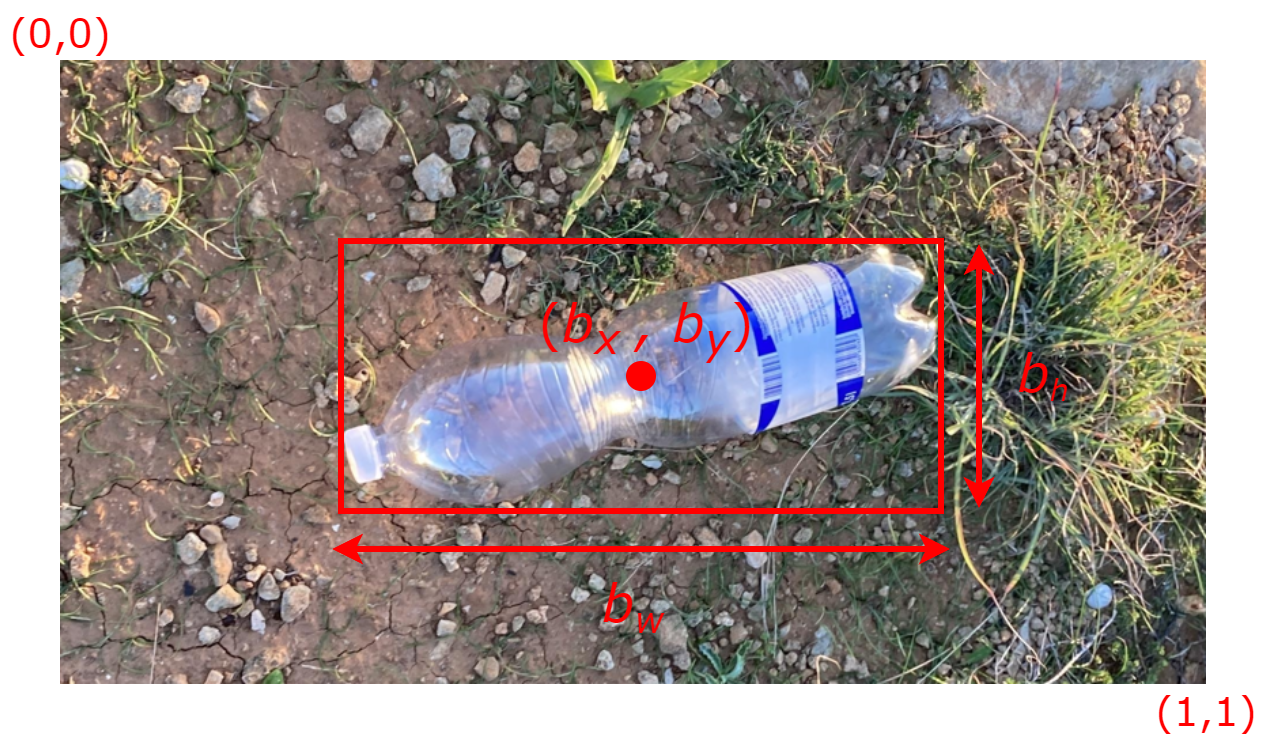
\includegraphics[width=0.7\columnwidth]{detection_explanation.png}
    \caption{Visual representation of the bounding box coordinate system on a modified image taken from the SODA dataset (Source: \cite{soda_dataset}).}
    \label{fig:detection_explanation}
\end{figure}

\subsection{Object Classification}
\label{subsec:2_classification}

While a bounding box indicates the location of an object, identifying the type of object detected is equally important. The result of the object classification task is usually presented as a label, which denotes the class or category assigned to the detected object from a predefined set of categories. Typically, alongside the label, the outputs from detection models also include a confidence score, indicating the degree of certainty that the object belongs to the assigned category \cite{od_2}. Figure \ref{fig:classification_explanation} provides a visual example of the classification and localisation tasks, illustrating multiple detections across different categories.

\begin{figure}[!htbp]
    \centering
    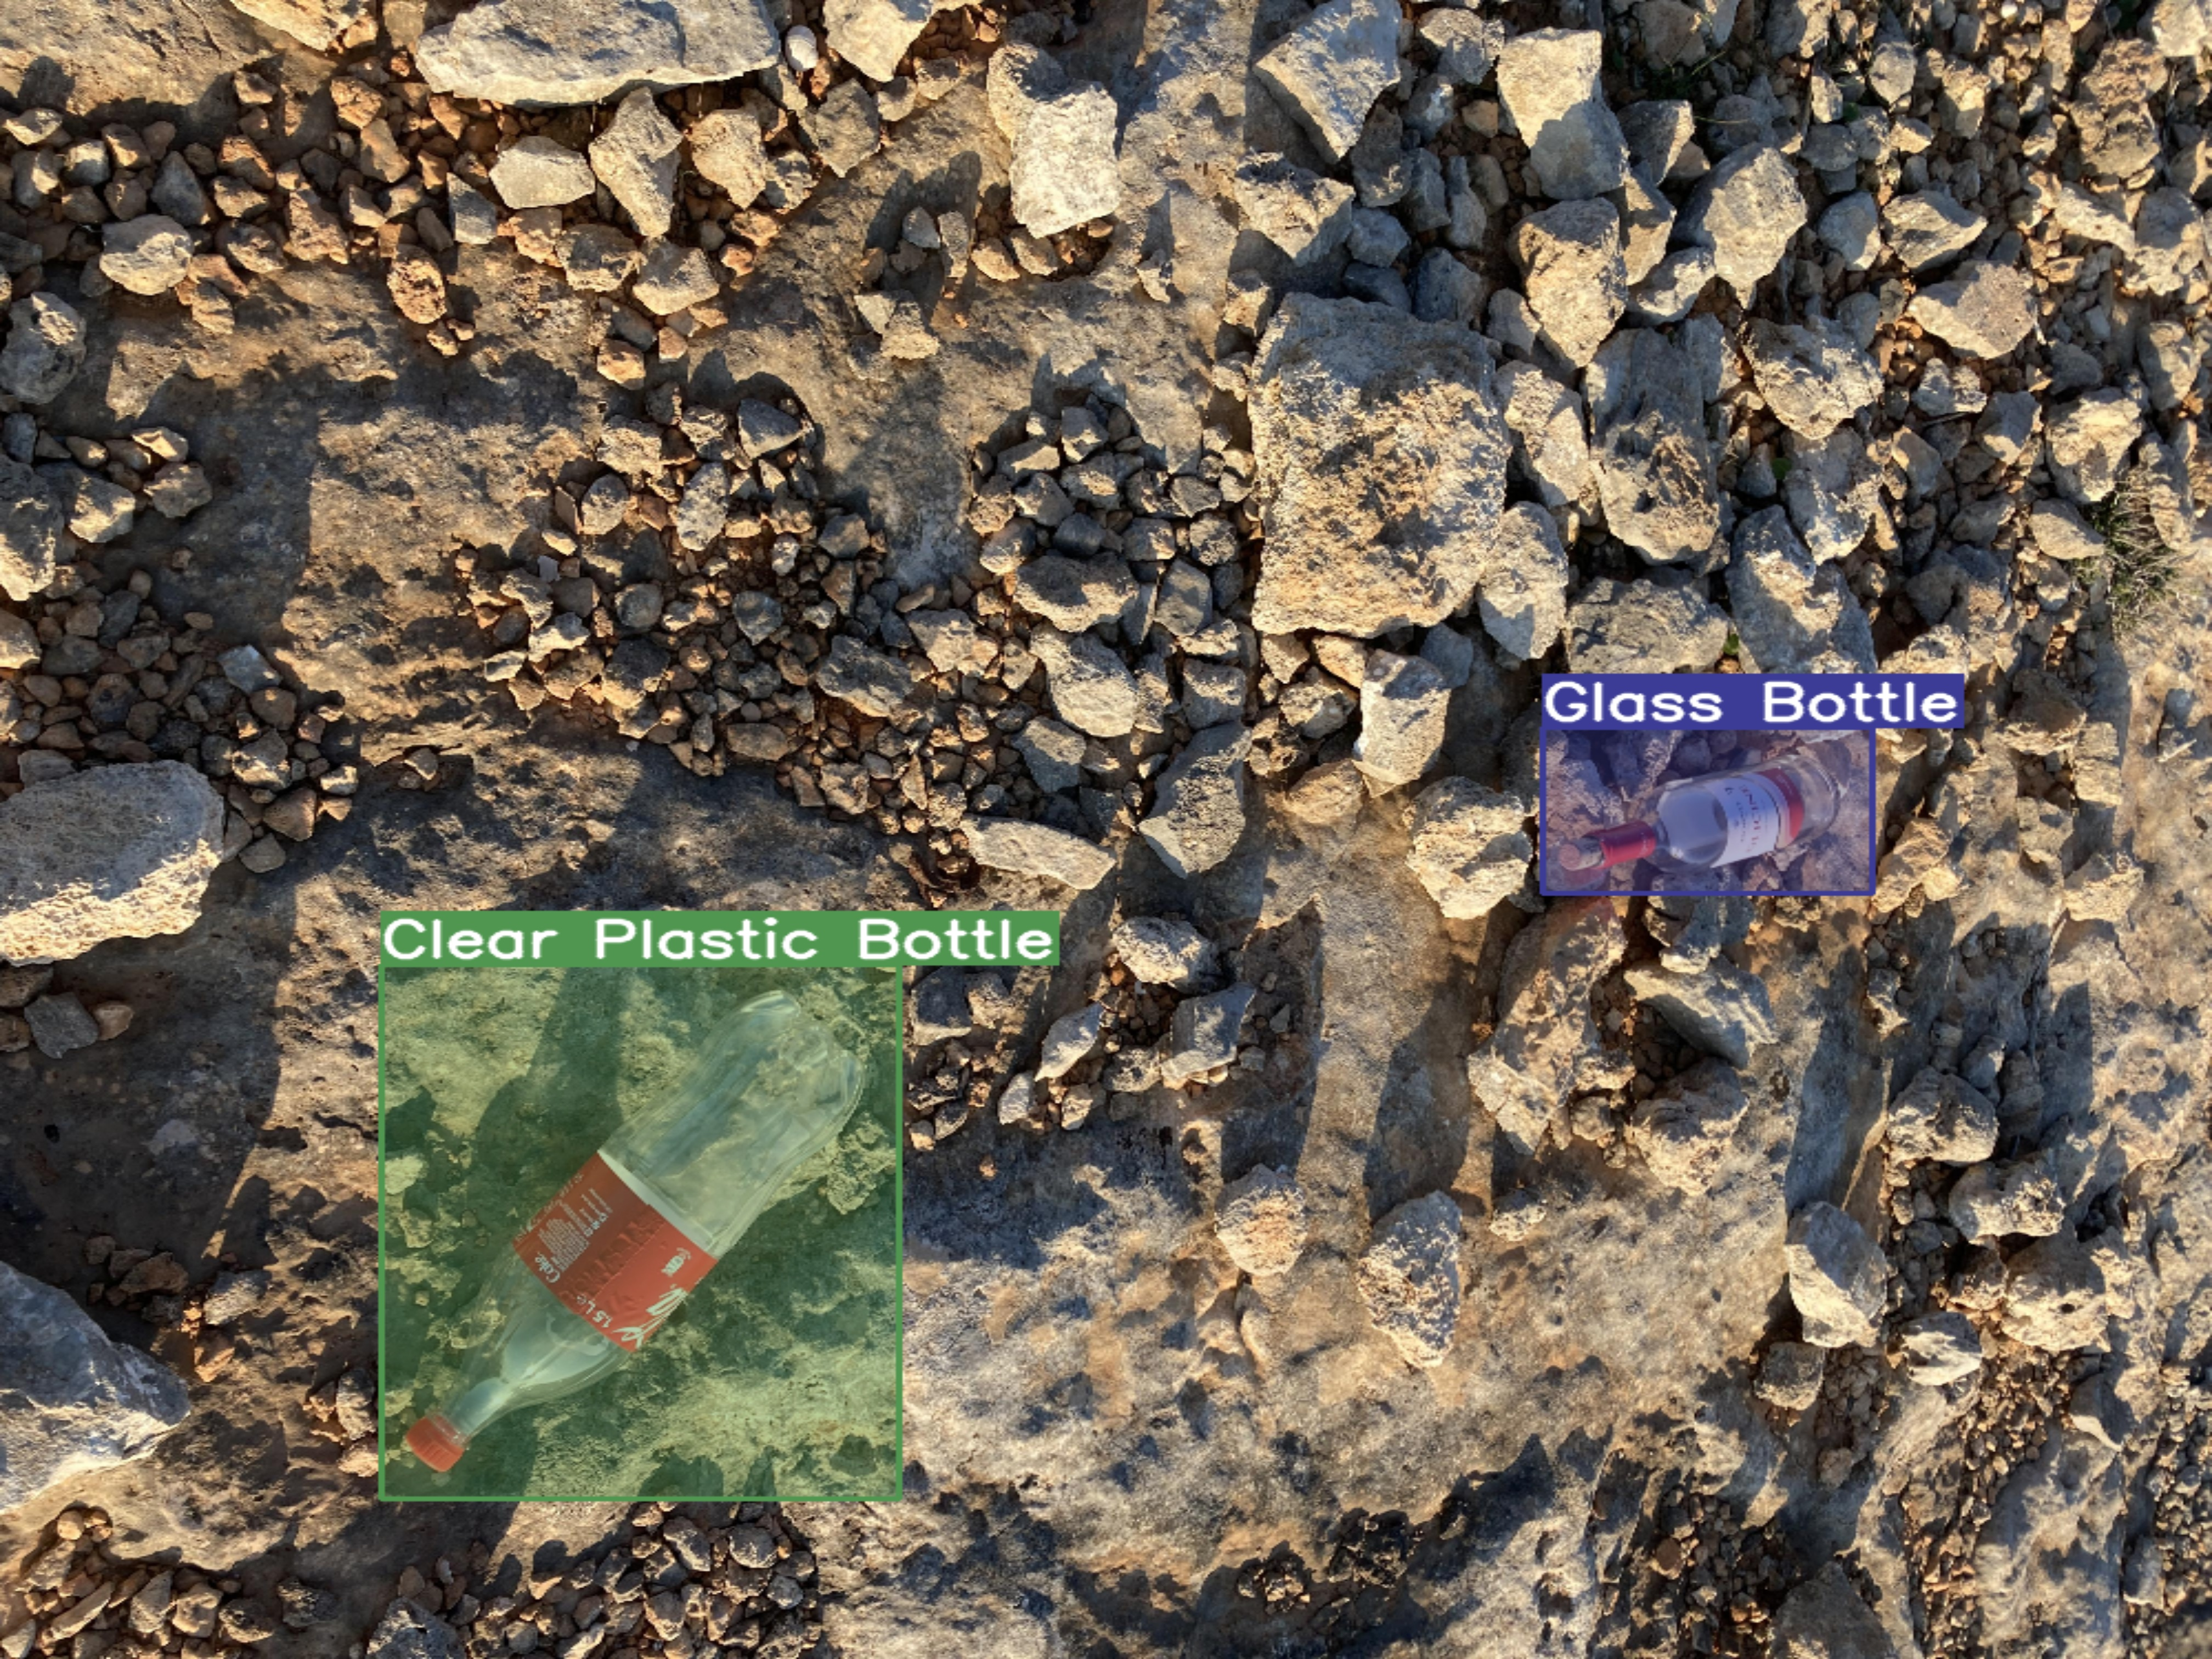
\includegraphics[width=0.7\columnwidth]{detection_soda.jpg}
    \caption{Visual representation of the classification and localisation tasks, showing multiple detections across various categories, based on an image from the SODA dataset (Source: \cite{soda_dataset}).}
    \label{fig:classification_explanation}
\end{figure}

\subsection{Challenges in Object Detection}
\label{subsec:2_challenges}

Although the object detection problem can be divided into two subproblems and may initially seem straightforward, it is far from simple. Developing models capable of robustly detecting multiple objects across a variety of images with diverse backgrounds is a highly complex task. Furthermore, it is crucial to consider the demands of computational efficiency and real-time performance, as these factors are integral to the practical application of detection models. As highlighted by \cite{od_survey_problems}, the object detection problem encompasses several key challenges:

\begin{enumerate}[label=\textbf{\arabic*.}]
    \item \textbf{Complex Backgrounds and Interferences}: In real-world situations, especially in outdoor environments, backgrounds tend to be complex and cluttered \cite{od_survey_problems, od_2}. Natural settings introduce factors such as weather conditions, lighting changes, shadows, and occlusions, which blur the distinction between objects and their surroundings, complicating the detection process \cite{four_pillars_od}. Furthermore, the wide range of object categories and shapes adds another layer of difficulty, as different detectors may categorise the same object in varying ways. In dynamic environments, objects within the same category can appear in different poses, necessitating that object detectors generalise effectively \cite{od_survey_problems}.

    \item \textbf{Scale Variability}: Objects in real-world images often appear at varying scales. For instance, in aerial imagery, litter may appear much smaller compared to close-up photographs. Additionally, the size disparity between different types of litter, such as a glass bottle and a cotton bud, further complicates detection. Designing an algorithm that can effectively manage multi-scale variations and generate multi-scale feature representations remains a significant challenge. To this end, such tasks typically require techniques like multi-scale input processing for robust detection \cite{od_survey_problems, four_pillars_od}.

    \item \textbf{Object Occlusion}: Object occlusion presents another common challenge in detection tasks and can be classified into \textit{partial occlusion} and \textit{complete occlusion} \cite{od_survey_problems, od_problem, survey_od_2}. Complete occlusion is particularly problematic, as it prevents the detector from extracting sufficient feature information, thus diminishing detection accuracy \cite{od_survey_problems}. In contrast, partial occlusion, while less severe, still results in parts of the object being obscured by noise, which leads to a loss of important feature information and a weaker feature representation.

    % \item \textbf{Computational Efficiency and Real-Time Performance}: Object detection models are often computationally intensive due to the large number of parameters involved. Achieving high detection speed while maintaining accuracy is an ongoing challenge, especially for real-time applications.  

    \item \textbf{Class Imbalance and Dataset Bias}: In supervised learning, object detection models rely on labelled datasets, where annotators identify object locations using bounding boxes. These labelled images are then employed to train the detection algorithm. However, datasets often suffer from class imbalances, with certain object categories being over-represented while others are under-represented. This imbalance can impair model performance, particularly when detecting less frequent objects \cite{od_survey_problems}. As noted by \cite{imbalance}, class imbalance manifests in two forms: \textit{foreground-background imbalance}, where background pixels dominate over object pixels, and \textit{foreground-foreground imbalance}, where some object categories are more prevalent than others. Both types of imbalance can hinder the model’s ability to accurately detect objects, especially in complex scenes \cite{od_survey_problems, imbalance}.

    \item \textbf{Small Object Detection}: Small objects occupy only a small number of pixels within an image, which makes it difficult for models to extract meaningful features. Accurate localisation is essential, as even minor deviations in bounding box predictions can result in detection failures \cite{od_survey_problems}. Furthermore, the limited feature representation of small objects, coupled with a lack of sufficient contextual information and an inadequate number of positive examples (\textit{foreground-background imbalance}), exacerbates the challenge of detecting such objects \cite{small_detection_survey, four_pillars_od}. 
\end{enumerate}

\subsection{Object Detection Before the Rise of Deep Learning}
\label{subsec:2_detection_pre_dl}

In efforts to address the object detection problem and its associated challenges, numerous approaches were developed using traditional and machine learning methods, preceding the widespread adoption of deep learning techniques.

\subsubsection{Traditional Methods}
\label{subsubsec:2_traditional}
% \noindent \textbf{Traditional Methods:}
Early methods for object detection were heavily reliant on creative heuristics and the efficiency of basic computational techniques. Simple strategies, such as background subtraction \cite{garcia2020background}, sought to identify objects by detecting fluctuations in pixel intensity across an image. As research progressed, more sophisticated feature-driven approaches emerged. One notable example was the development of Haar cascade classifiers \cite{vinh2020real, javed2022human}, designed particularly for face detection. These classifiers exploited Haar-like features, which captured essential edge and line structures within images.
Another prominent method introduced at the time was the \gls{hog} descriptor \cite{dalal2005histograms, bhattarai2023histogram}, which was widely applied to tasks such as pedestrian detection. \gls{hog} focused on the distribution of local gradient directions, capturing the shape and appearance of objects through structured edge information.

Alongside these developments, several feature extraction techniques became foundational. The \gls{sift} \cite{lowe2004distinctive} algorithm identifies distinctive keypoints within an image by detecting local extrema in a scale-space constructed from \gls{dog}, allowing for reliable feature matching under variations in scale and rotation. The \gls{surf} algorithm \cite{bay2006surf} built upon these ideas, offering a faster alternative while maintaining reliable performance under transformations such as viewpoint and illumination changes.
Later, the \gls{orb} algorithm \cite{rublee2011orb} emerged, combining the efficiency of the \gls{fast} keypoint detector with the compactness of the \gls{brief} descriptor. \gls{orb} provided a computationally inexpensive, rotation-invariant solution, serving as a competitive alternative to \gls{sift} and \gls{surf} in environments requiring faster performance.

\subsubsection{Machine Learning Approaches}
\label{subsubsec:2_machine_learning}

In tandem with traditional methods, notable advances in object detection were made through the adoption of \gls{ml}, a branch of \gls{ai} focused on enabling systems to learn patterns from data \cite{machine_learning}. During this period, \gls{svms} \cite{hearst1998support} emerged as a pivotal tool, providing a strong classification framework, particularly when combined with feature descriptors such as \gls{hog} \cite{bhatt2023state}. Other machine learning strategies also contributed meaningfully to the field's development. Boosting algorithms, such as \gls{adaboost}, proved instrumental in the Viola-Jones face detection framework \cite{viola2001rapid}, while ensemble methods, including \gls{rf} \cite{saffari2009line} and techniques utilising \gls{rgbd} information \cite{seychell16}, further expanded detection capabilities. Although these approaches improved performance by allowing models to learn directly from data, they continued to rely heavily on manually engineered features. Additional progress was marked by the introduction of \gls{dpm} \cite{felzenszwalb2009object}, which conceptualised objects as collections of interconnected parts, thus enabling more effective modelling of variations in object appearance. Collectively, these machine learning-based methods significantly advanced object detection, laying the essential foundations for the subsequent development of deep learning approaches.

\subsection{Object Detection in the Era of Deep Learning}
\label{subsec:2_detection_in_dl}

The introduction of \gls{dl}, most notably \gls{cnn}, brought about a fundamental shift in the field of object detection \cite{cnn_survey}. In contrast to earlier methods that depended heavily on labour-intensive, hand-crafted feature engineering, \gls{cnn} are capable of automatically extracting features from large datasets, thereby streamlining the detection process and improving overall efficiency \cite{feature_learning, deep_learning_review, cnns}. This progression led to the development of a new generation of object detectors that demonstrated greater accuracy and reliability than their traditional counterparts. Consequently, numerous object detection architectures have been introduced, each offering distinct advantages and facing particular limitations.

CNN-based object detectors are generally categorised into two principal types: one-stage detectors and two-stage detectors \cite{one_two_stage_detection}. More recently, transformer-based models, originally proposed for natural language processing tasks \cite{transformers}, have been successfully adapted for computer vision applications, including object detection \cite{detr, rt-detr}, pushing performance boundaries even further. Beyond these mainstream approaches, emerging deep learning models increasingly incorporate visual attention mechanisms to strengthen feature representation and contextual reasoning within images \cite{bartolo2024correlationobjectdetectionperformance, va_detection}. Moreover, alternative paradigms, such as \gls{rl}, have also been explored to dynamically optimise object detection strategies \cite{bartolo2024integratingsaliencyrankingreinforcement, Caicedo_2015_ICCV}.

% In the sections that follow, we review one-stage detectors, two-stage detectors, transformer-based detectors, as well as approaches that do not fit neatly within these established categories.

\subsubsection{One Stage Detectors}
\label{subsubsec:2_onestage}

One-stage detectors address the problem of object detection by concurrently performing localisation and classification within a single network, predicting bounding boxes and corresponding labels in a single forward pass.
OverFeat \cite{overfeat}, introduced in 2013, marked an early application of deep learning to object detection. It employed a multi-scale sliding window method wherein a classifier generated class labels and confidence scores at each spatial location. Prediction quality was subsequently improved through adjustments in resolution and the merging of bounding boxes.

The You Only Look Once (YOLO) series significantly reshaped one-stage detection by reframing object detection as a regression problem. The original \gls{yolo} model \cite{yolo}, released in 2016, partitioned images into an $S \times S$ grid, with each cell responsible for predicting bounding boxes, confidence scores, and class probabilities (refer to Figure \ref{fig:yolov1}). Later versions introduced several refinements: \gls{yolo}v2 \cite{yolov2} integrated batch normalisation and optimised anchor boxes; \gls{yolo}v4 \cite{yolov4} adopted a suite of training techniques commonly referred to as bag-of-freebies \cite{bagoffreebies}; \gls{yolo}v5 \cite{yolov5} incorporated automatic anchor learning; and \gls{yolo}X \cite{yolox} shifted towards anchor-free methodologies. More recently, \gls{yolo}v12 \cite{yolov12} introduced attention-driven designs, leveraging linear attention mechanisms and residual-efficient layer aggregation networks.

Further adaptations have continued to emerge. For example, \gls{yolo}-NAS \cite{yolonas} improved detection efficiency by employing \gls{nas} within a quantisation-friendly framework. Meanwhile, \gls{yolo}-World \cite{yoloworld} extended the model’s capabilities to open-vocabulary detection, integrating vision-language path aggregation and region-text contrastive loss, achieving notable gains in both speed and accuracy over contemporary models.

\begin{figure}[ht]
    \centering
    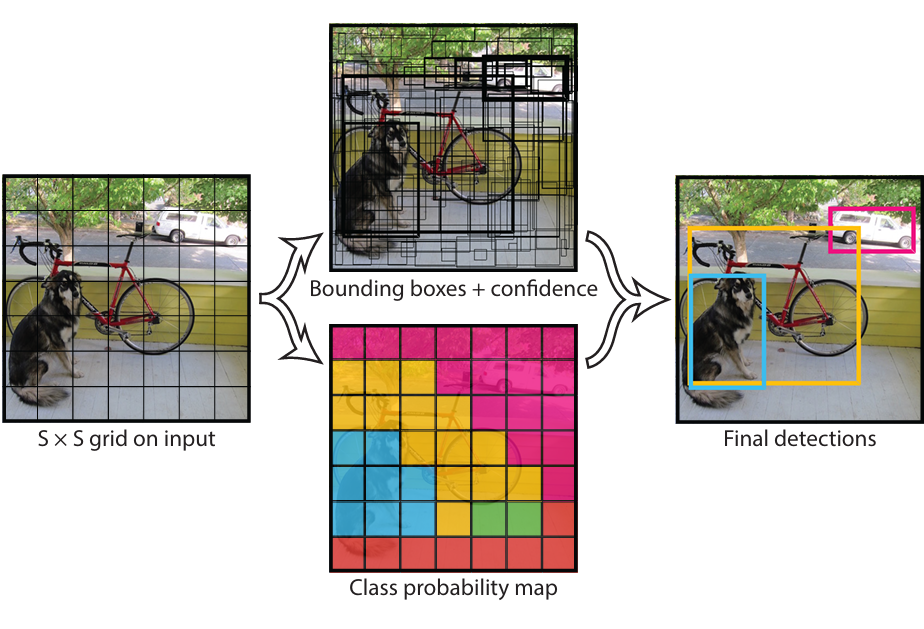
\includegraphics[width=0.7\linewidth]{yolov1.png}
    \caption{YOLOv1 pipeline. (Source: \cite{yolo})}
    \label{fig:yolov1}
\end{figure}

In parallel with developments in \gls{yolo}, other notable one-stage detectors have emerged. The \gls{ssd} Detector \cite{ssd}, introduced in 2016, employed default bounding boxes with a variety of aspect ratios and multi-scale feature maps, enabling it to handle objects of varying sizes. RetinaNet \cite{retinanet} addressed the issue of class imbalance through the application of \textit{Focal Loss}, incorporating a ResNet backbone along with a \gls{fpn} \cite{fpn} for enhanced multi-scale feature extraction. The \gls{fcos} model  \cite{fcos} adopted a fully convolutional architecture, directly predicting centre points and bounding boxes without relying on region proposals.

\subsubsection{Two Stage Detectors}
\label{subsubsec:2_twostage}

In contrast to one-stage detectors, two-stage detectors tackle object detection by decoupling localisation and classification into distinct stages, each handled by separate networks.
The \gls{rcnn} family was instrumental in establishing the two-stage framework. This began with the original \gls{rcnn} model \cite{rcnn}, introduced in 2014, which utilised AlexNet \cite{alexnet} as its backbone and relied on selective search to identify potential object regions. This approach was subsequently refined through Fast \gls{rcnn} \cite{fastrcnn}, which bolstered efficiency by processing the entire image once to generate a feature map, before applying selective search. A more significant breakthrough came with Faster \gls{rcnn} \cite{fasterrcnn}, which introduced the \gls{rpn}, effectively eliminating the need for selective search. The \gls{rpn} enabled the network to directly learn region proposals through the use of anchor boxes of various scales and aspect ratios (see Figure \ref{fig:fasterrcnn}). Finally, Mask \gls{rcnn} \cite{maskrcnn} extended the Faster \gls{rcnn} architecture by incorporating an additional branch that predicted segmentation masks for each \gls{roi}.

\begin{figure}[ht]
    \centering
    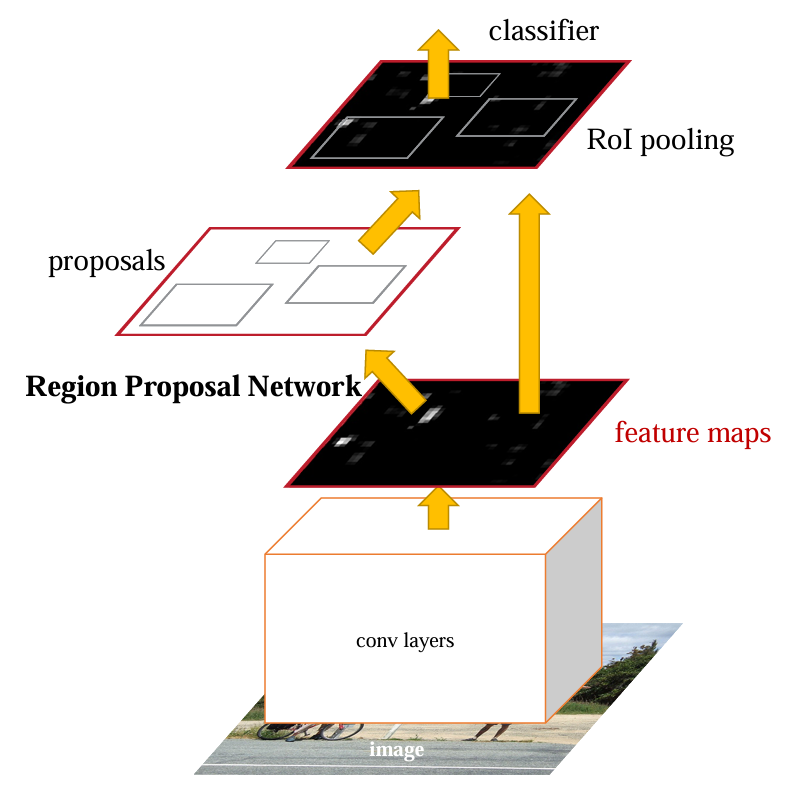
\includegraphics[width=0.5\linewidth]{fasterrcnn.png}
    \caption{Faster R-CNN pipeline. (Source: \cite{fasterrcnn})}
    \label{fig:fasterrcnn}
\end{figure}

Complementing these technological advancements, \gls{fpn} \cite{fpn} improved detection across all network layers by constructing a feature pyramid for improved multi-scale detection. This pyramid included bottom-up pathways that captured semantic information and top-down pathways that refined these maps by merging high-level features with spatially rich information. \gls{rfcn} \cite{rfcn} integrated both classification and localisation tasks, utilising position-sensitive score maps to classify and refine bounding box coordinates. This approach struck a balance between speed and accuracy by enabling shared computation across regions.
Building on these two-stage frameworks, EfficientDet \cite{efficientdet} incorporated an EfficientNet \cite{efficientnet} backbone and employed a weighted bi-directional feature pyramid network for efficient multi-scale feature fusion. Furthermore, it introduced a compound scaling method that uniformly scaled resolution, depth, and width across the backbone, feature network, and prediction networks.

\subsubsection{Transformer-Based Detectors}
\label{subsubsec:2_transformers}

Transformers, originally developed for natural language processing \cite{transformers}, have garnered significant attention in computer vision \cite{visiontransformer}, especially for object detection tasks. The \gls{detr} \cite{detr}, introduced in 2020, marked a pioneering shift in transformer-based object detection by framing the task as a set prediction problem. \gls{detr} removed the need for region proposals, employing a bipartite matching loss that aligns predicted boxes with ground-truth boxes. Its encoder-decoder architecture processes input data through self-attention mechanisms, enabling it to effectively distinguish individual instances. This structure supports both object detection and panoptic segmentation tasks (see Figure \ref{fig:detr}).

\begin{figure}[ht]
    \centering
    \includegraphics[width=0.9\linewidth]{detr.png}
    \caption{DETR architecture. (Source: \cite{detr})}
    \label{fig:detr}
\end{figure}

Several models have built upon the foundation laid by \gls{detr}. The \gls{dino} framework \cite{zhang2022dino, li2022dn, liu2022dabdetr} improved both training efficiency and overall performance. Grounding \gls{dino} \cite{groundingdino} advanced zero-shot object detection by enabling the identification of objects without prior training on specific categories. This was achieved through the use of natural language queries and the multimodal fusion of textual and visual information.
Real-time transformer-based detection has also emerged as a significant advancement. \gls{rtdetr} \cite{rt-detr} addressed the limitations of non-maximum suppression by incorporating a hybrid encoder and high-quality initial queries. This made the model more efficient and adaptable, eliminating the need for retraining. \gls{rtdetr}v2 \cite{rt-detrv2} further optimised training strategies and integrated bag-of-freebies techniques, enhancing real-time performance.

Vision-language models have also adopted transformer architectures for object detection. PaliGemma \cite{paligemma} combined a vision transformer for image encoding with a transformer decoder to merge textual and visual data, framing object detection as a set prediction task. Its successor, PaliGemma 2 \cite{paligemma2}, improved efficiency by incorporating Gemma 2 language models with the SigLIP vision encoder, enabling it to handle multiple input resolutions more effectively. Similarly, Florence-2 \cite{florence2} utilised a unified, prompt-based architecture with an image encoder and a multi-modality encoder-decoder to address a range of vision-language tasks, including object detection, captioning, and segmentation.
These transformer-based approaches collectively represent a paradigm shift in object detection, offering end-to-end solutions that eliminate traditional components, such as non-maximum suppression, while enabling more flexible, multimodal, and zero-shot capabilities.

\subsubsection{Other Deep Learning Approaches}
\label{subsubsec:2_other_approaches}

Deep learning methodologies that go beyond traditional one-stage, two-stage, and transformer detectors have emerged to tackle specific challenges in object detection. These approaches can be categorised based on their underlying principles and technical innovations.
One prominent paradigm is reinforcement learning-based detection frameworks, starting with the approach by Caicedo et al. \cite{Caicedo_2015_ICCV}, which used class-specific Deep Q-Network agents to iteratively refine object localisation by framing detection as a \gls{sdmp}. Subsequent studies have expanded on this foundation by incorporating multitask learning \cite{multitask_learning}, integrating saliency ranking \cite{bartolo2024integratingsaliencyrankingreinforcement}, and developing other complementary strategies \cite{reinforcenet, bar_rl} to enhance the reinforcement learning paradigm for object detection.

Feature enhancement techniques represent another significant area, exemplified by \gls{dcn} introduced in 2017 \cite{dcn}. \gls{dcn} improves feature extraction across various detector architectures by incorporating deformable convolutional layers and \gls{roi} pooling, enabling adaptive sampling of input features with learnt offsets. This approach better models spatial transformations and bolsters the detection of objects with varying shapes and sizes.
Point-based and slicing-based approaches offer alternative detection paradigms. CenterNet \cite{centernet} models objects as single points (the centres of their bounding boxes) and uses keypoint estimation to identify these centres while regressing to other properties such as size and orientation. This results in an end-to-end differentiable system that is simpler, faster, and often more accurate than traditional bounding box-based detectors. The \gls{sahi} framework \cite{sahi_detection} improves small object detection by dividing input images into overlapping patches during both fine-tuning and inference. This increases pixel coverage for small objects, which are then reassembled through non-maximum suppression.
These diverse approaches complement mainstream detection architectures by addressing specific limitations and introducing novel perspectives on the object detection problem.


\section{Learning Using Privileged Information}
\label{subsec:2_lupi_background}

Unlike the conventional machine learning approach, which selects the most suitable function from a predefined set based solely on input-output training examples, the Learning Using Privileged Information (\gls{lupi}) paradigm introduces a richer structure. Proposed by V. Vapnik and A. Vashist \cite{lupi, Vapnik2015LearningUP}, the \gls{lupi} framework incorporates additional information during the training phase. This information, which is not available at test time, is intended to accelerate the convergence of the learning process.
\gls{lupi} is inspired by human learning, reflecting the idea that a single day with a great teacher can be more valuable than a thousand days of independent study \cite{lupi_distillation, lupi}. Following the intuition that a student gains more than just examples, the teacher provides explanations, comparisons, and context, which enhance understanding \cite{lupi, lupi_distillation, lupi_nips}.
In much the same way, \gls{lupi} incorporates additional information, known as privileged information (\gls{x_star}), during training. This data, which is not available during testing, offers a deeper understanding beyond the standard input-output $($\gls{x}$ ,$ \gls{y}$)$ pairs. 
As outlined in \cite{lupi}, the standard supervised learning framework is formally expressed by a training set composed of input-output pairs:
\begin{equation} \label{eq:supervised_learning}
(x_1, y_1), \dots, (x_l, y_l), \quad x_i \in X, y_i \in Y  .
\end{equation}

\noindent Assuming that the data pairs $($\gls{x}$ ,$ \gls{y}$)$ are generated according to a fixed but unknown probability distribution \(P(x, y)\). The task is to select the function \(\hat{y} = f(x; \theta^{*})\), with parameter \(\theta^{*} \in \Theta\), from a specified class of functions which minimises the probability of misclassification. In this setting, the input vector \(x_i \in X\) describes an instance, and \(y_i\) denotes its corresponding target label. The predicted output \(\hat{y}\) is the model's estimate of the true label \(y\) given the input \(x\).
In comparison, within the \gls{lupi} framework, training data can be represented as a sequence of triplets:
\begin{equation} \label{eq:lupi_pairs}
(x_1, x_1^*, y_1), \dots, (x_l, x_l^*, y_l), \quad x_i \in X , x_i^* \in X^*, y_i \in Y .
\end{equation}

\noindent These samples are assumed to be drawn from an unknown but fixed probability distribution \( P(x, x^*, y) \). The task is to select, from a specified class of functions \( f(x, \theta) \), where \( \theta \in \Theta \), the function \( y = f(x, \theta^*) \) that minimises the probability of classification errors.
Although the aim remains the same as in the conventional supervised learning setting, the \gls{lupi} paradigm introduces an additional element during training. Rather than learning from pairs \( (x, y) \), the model receives triplets \( (x, x^*, y) \), where \( x^* \in X^* \) represents privileged information. This privileged component belongs to a separate space \( X^* \), which need not coincide with the original input space \( X \).

In addition, the \gls{lupi} framework can be extended to align with the concept of knowledge distillation \cite{hinton_distillation}, as proposed in \cite{lupi_distillation}. Both approaches can be viewed as instances of a broader idea in which one model provides guidance to another, a process referred to as \textit{generalised distillation}. This unified perspective treats Hinton’s distillation \cite{hinton_distillation} and Vapnik’s use of privileged information \cite{lupi} as complementary forms of machine-driven instruction.
In this framework, a teacher model is first trained on standard input-output $($\gls{x_star}$ ,$ \gls{y}$)$  pairs. The teacher then produces soft labels, which act as enriched supervisory signals. These soft labels are used in Hinton’s distillation method to train a student model. The student learns from the soft labels generated by the teacher, benefiting from the additional information embedded in the teacher’s predictions, even though it only receives standard input-output $($\gls{x}$ ,$ \gls{y}$)$  pairs \cite{lupi_distillation}.

% -- Start of Lit Review --

\section{Review of Litter Detection Methodologies}
\label{sec:3_litter}

Within the broader context of object detection, the task of identifying litter poses particular challenges, especially when employing an \gls{uav} to capture expansive outdoor scenes. The difficulty lies in the nature of the environments: litter often appears amid textured and irregular backgrounds such as rocky outcrops or dense vegetation, where visual contrast is minimal \cite{small_litter_detection, taco2020, plastopol}. Despite these difficulties, several studies have addressed this problem by creating a dataset or proposing varied and increasingly refined approaches. In what follows, the review concentrates on the most prominent and widely cited works, offering a representative view of the prevailing methodologies adopted in recent research.

\subsection{Bottle Detection in the Wild Using Low-Altitude UAVs}
\label{subsec:3_bdw}

To address the challenge of bottle detection, the \gls{bdw} dataset, introduced in 2018, was developed to identify plastic bottles across varied environments using \gls{uav} imagery, with the broader aim of supporting recycling initiatives. The dataset comprises of images captured from a DJI Phantom 4 Pro quadcopter equipped with a 3-axis stabilised gimbal. The footage was taken at \gls{agl} altitudes ranging from 10 to 30 metres, with a resolution of $5472 \times 3078$ pixels. 
To bolster dataset diversity and simulate real-world conditions, the dataset includes images featuring eight distinct background types: bush forest land, step, flat land, sand land, wasteland, mixture, plastic stadium, and grassland, as illustrated in Figure \ref{fig:bdw}. This diversity of different backgrounds, presented as part of the dataset engineering process, accounts for the complexities associated with varied backgrounds in terms of generalising to real-world data. Furthermore, the authors highlight that the plastic bottles in the dataset are relatively small, with sizes less than $50 \times 50$ pixels, and are often transparent, which allows the background to be visible through the bottles, thereby significantly increasing the detection difficulty \cite{bdwdataset}.

\begin{figure}[!htbp]
    \centering
    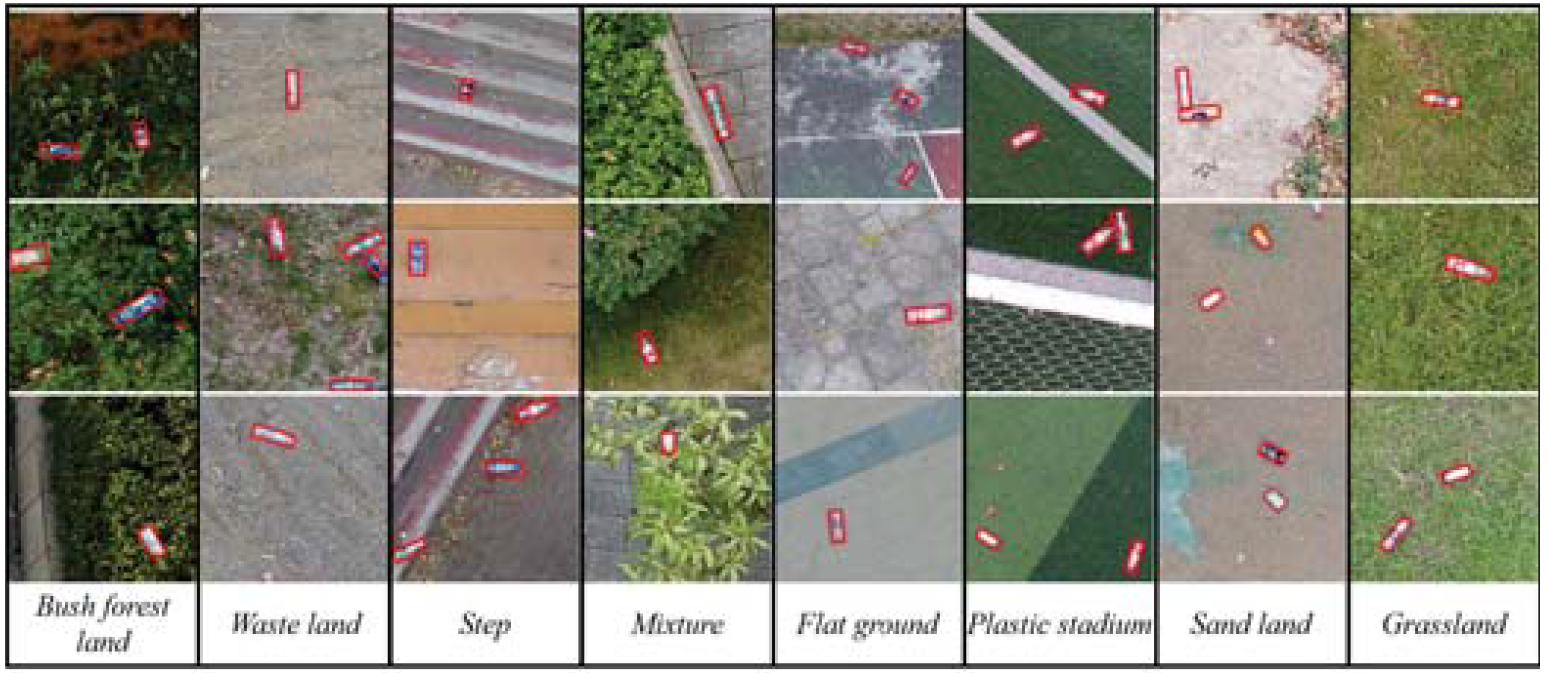
\includegraphics[width=0.9\linewidth]{BDWDataset1.png}
    \caption{Showcasing the different backgrounds found in the BDW dataset. (Source: \cite{bdwdataset})}
    \label{fig:bdw}
\end{figure}

The \gls{bdw} dataset contains 25,407 annotated images with 34,791 object instances, all belonging to a single category: \textit{plastic bottles}. Annotations in the \gls{bdw} dataset utilise \gls{obbs}, which include traditional bounding box coordinates along with additional parameters: centre coordinates ($c_x$, $c_y$), height ($h$), width ($w$), and orientation angle ($\theta$), where $\theta$ represents the angle from the horizontal axis. Additionally, the dataset was split randomly into training (64\%), validation (16\%), and testing (20\%) subsets \cite{bdwdataset}.

In their study, the authors utilise the created \gls{bdw} dataset in multiple experiments to train popular object detection models, including Faster \gls{rcnn}, \gls{ssd}, \gls{yolo}v2, and a Modified \gls{rrpn} from \cite{rrpn}. Among these models,  \gls{rrpn} uniquely predicts \gls{obbs}, whereas the others predict standard axis-aligned bounding boxes. Wang et al. report that these experiments demonstrate that OBB regression is crucial for oriented object detection. In addition,  \gls{rrpn} achieved superior localisation accuracy while minimising false alarms and false positives, making it the most robust model in the study \cite{bdwdataset}.

\subsection{Optimising Beached Litter Monitoring through Aerial Imagery}%UM Geo. Survey
\label{subsec:3_geosurvey}

Building on the concept of litter detection proposed by \cite{bdwdataset}, Deidun et al. (2018) introduced an optimised system for monitoring beach litter through aerial imagery \cite{umgeosurvey}. Their study focused on three coastal stretches within the North-East Marine Protected Area of the Maltese Islands. The monitored areas included Baħar iċ-Ċagħaq, specifically the western and eastern flanks of its rocky peninsula. 
The data collection process utilised a DJI Phantom 4 Pro drone, configured with a gimbal angle of -90 degrees and flown at an \gls{agl} altitude of 30 metres. This altitude was empirically determined to balance image quality and spatial resolution, following tests conducted at heights ranging from 20 to 50 metres. Images were captured at varying ground resolutions, ranging from 2.5 to 50 centimetres per pixel, to provide detailed visual data \cite{umgeosurvey}.

The collected footage was processed using OpenDroneMap software \cite{OpenDroneMap}, which facilitated the creation of point clouds and texture maps. Georeferenced orthophoto maps with a resolution of 1 centimetre per pixel were generated using \gls{gps} metadata embedded in the \gls{exif} data of each image file. These orthophotos were subsequently tiled and visualised in Google Earth© \cite{umgeosurvey}.

\begin{figure}[!htbp]
    \centering
    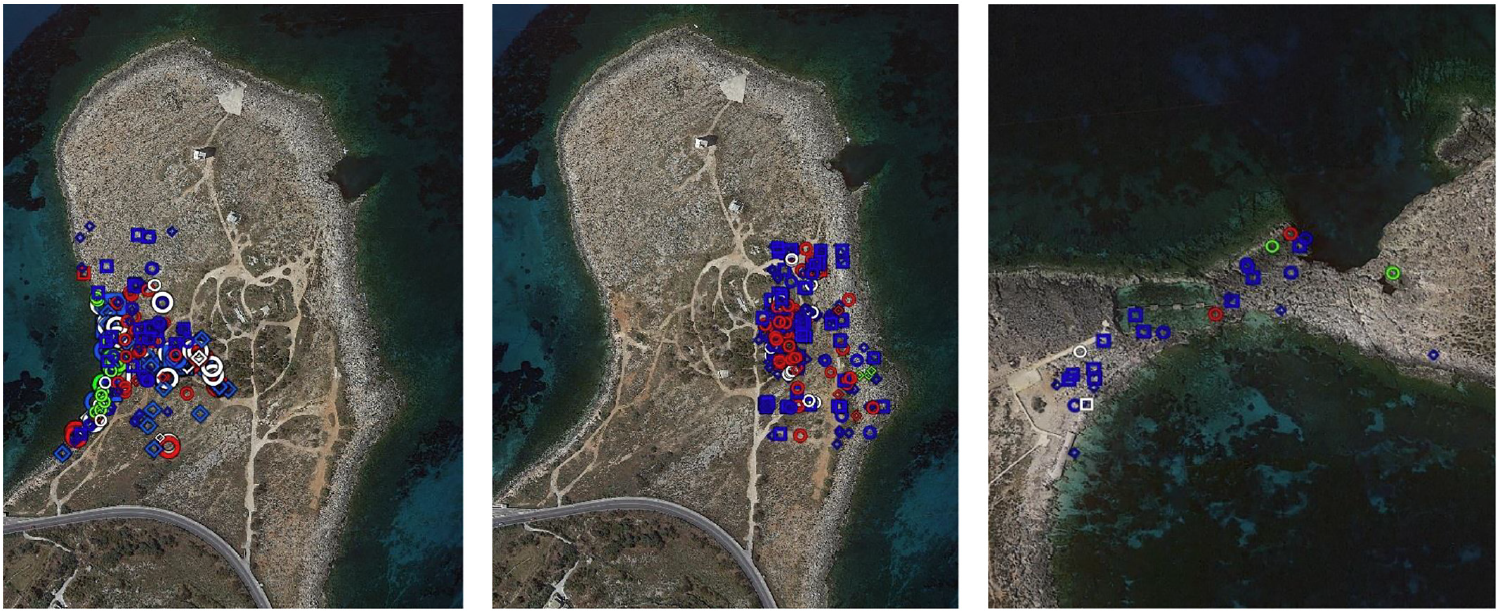
\includegraphics[width=1\linewidth]{UMgeosurvey.png}
    \caption{Showcasing snapshots from the digitised marine litter database, highlighting litter detected in the west (left) and east (middle) bays of Baħar iċ-Ċagħaq, and Qawra Point (right). Legend: blue = plastics; green = rope; red = wood; black = rubber; white = other non-natural materials. (Source: \cite{umgeosurvey})}
    \label{fig:geosurvey}
\end{figure}

The digitised database of detected marine litter, shown in Figure \ref{fig:geosurvey}, was created using 473 annotated images containing 608 labelled instances of litter. These instances were categorised into five litter types: \textit{plastics, rope, wood, rubber, and non-natural items}. While the study did not involve testing object detection algorithms, its key contribution lies in presenting a robust data collection protocol \cite{umgeosurvey}.

\subsection{SuperDock: Automated Floating Trash Monitoring System}
\label{subsec:3_superdock}

To address the environmental issue of trash in rivers, Niu et al. (2019) proposed an automated river trash monitoring system called SuperDock \cite{superdock}. This system consists of a \gls{rpu}, a docking station, and a \gls{uav}. SuperDock enables the \gls{uav} to land precisely on the docking station, where automated battery replacement is performed. This allows the \gls{uav} to resume its monitoring tasks without significant wasted time. SuperDock incorporates a deep learning-based trash detection module, leveraging the \gls{yolo}v3 architecture. As illustrated in Figure \ref{fig:superdock}, the system includes three key components: the \gls{rpu}, the docking station, and the \gls{uav}. The object detection process uses data collected from a consumer-grade \gls{uav} flying at an \gls{agl} altitude of 5 to 10 meters \cite{superdock}.

\begin{figure}[!htbp]
    \centering
    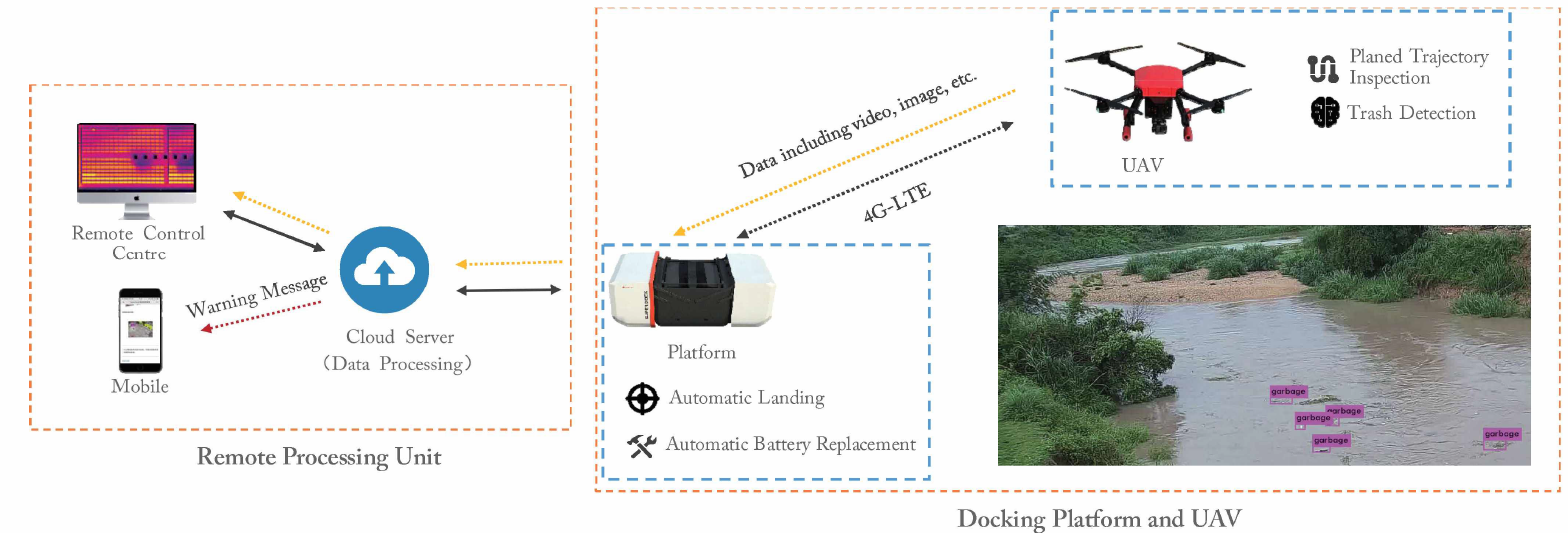
\includegraphics[width=0.9\linewidth]{superdock.png}
    \caption{Block diagram of the automated SuperDock system. (Source: \cite{superdock})}
    \label{fig:superdock}
\end{figure}

The dataset features 100 annotated images, divided into 80\% for training and 20\% for testing, with a total of 312 object instances. All types of litter in the dataset are annotated under a single category: \textit{garbage}. Data augmentation techniques were applied, increasing the dataset size by a factor of five. Additionally, the authors used Microsoft AirSim (Aerial Informatics and Robotics Simulation) to experiment with the gathered data. The dataset was used to train and test three object detection models: Faster \gls{rcnn}, \gls{yolo}v3, and \gls{yolo}v3 with an improved loss function. Among these, the improved \gls{yolo}v3 model demonstrated the best performance in terms of both accuracy and processing time. While the study did not focus on creating a specialised litter detection dataset, its primary contribution lies in developing an automated trash monitoring system \cite{superdock}.

\subsection{Detection and Monitoring of Styrofoam Litter using UAV Imagery}%Styrofoam Monitoring
\label{subsec:3_styrofoam}
To analyse the patterns of waste generation and distribution, as well as the factors contributing to its inflow, Bak et al. (2019) proposed an automated floating trash monitoring system based on deep learning \cite{styrofoam}. Their study focused on Heungnam Beach in Geoje, situated in Korea’s marine climate zone on the South Sea. The system utilises SegNet \cite{segnet}, an instance segmentation model based on a convolutional encoder-decoder structure developed by the University of Cambridge, to detect beach litter.
While the authors did not specify the exact number of annotated images in the dataset, \gls{uav} imagery was collected using DJI's MAVIC 2 PRO, a multi-rotor \gls{uav}. The \gls{uav} operated at an altitude of 15 meters, chosen to account for the size of the beach litter and the \gls{gsd}. Orthoimages were generated using Pix4D and divided into $224 \times 224$-pixel segments for neural network input, with positional information recorded for each segment \cite{styrofoam}.

\begin{figure}[!htbp]
    \centering
    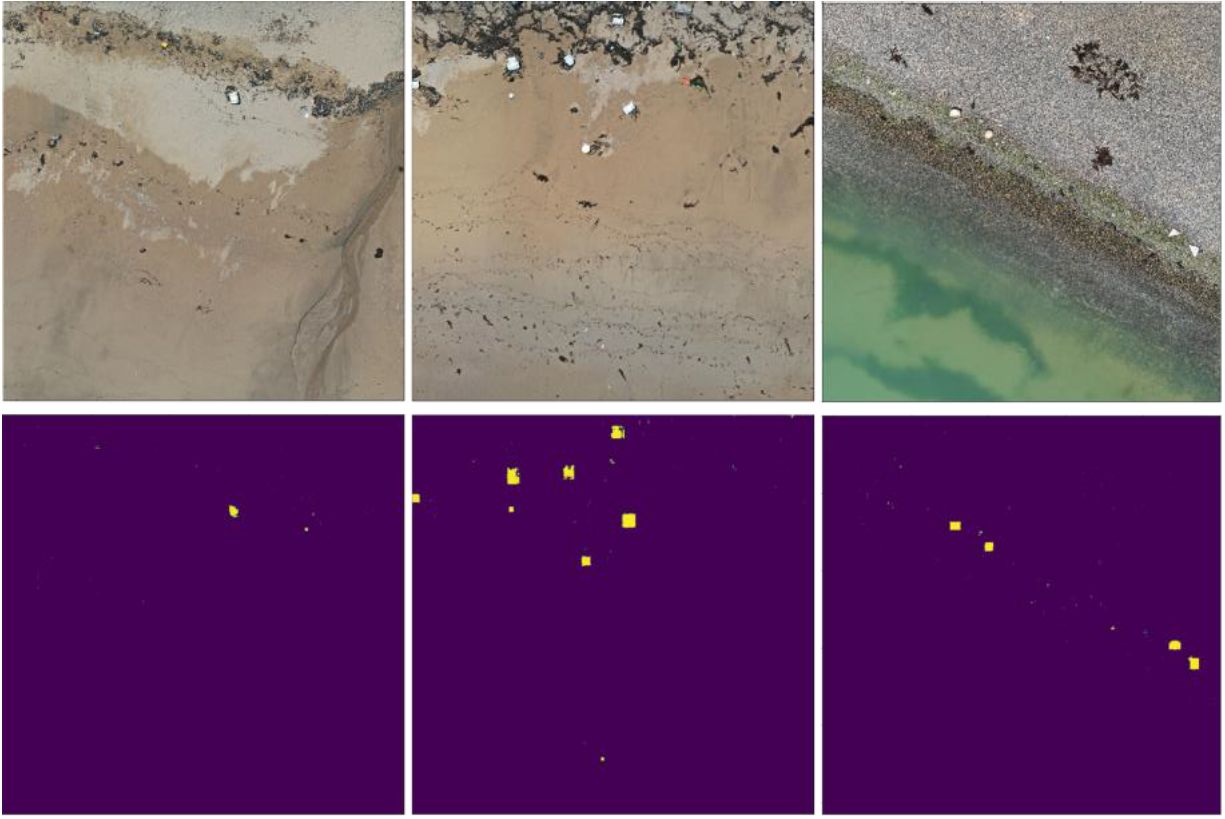
\includegraphics[width=0.8\linewidth]{styrofoam.png}
    \caption{Styrofoam detection results using the trained neural network. (Source: \cite{styrofoam})}
    \label{fig:styrofoam}
\end{figure}

The developed dataset only contained a single litter category, focusing on detecting \textit{Styrofoam} waste, and was notably imbalanced, as the majority of pixels represented the background, with less than 5\% occupied by detected objects. To mitigate this imbalance, data augmentation techniques were employed. Despite these challenges, the system achieved an impressive detection accuracy of 98.2\%, demonstrating its efficacy in identifying Styrofoam litter on beaches, as depicted in Figure \ref{fig:styrofoam} \cite{styrofoam}.

\subsection{Small Litter Detection in Highly Variable Backgrounds}
\label{subsec:3_smalldetection}

In 2019, Schembri and Seychell proposed a case study focusing on litter detection through aerial imagery to address challenges in small object detection in highly variable backgrounds \cite{small_litter_detection}. This study explored techniques for small object localisation using \gls{cnn} to detect litter in outdoor, non-urban imagery. The dataset for this research was collected using a consumer-grade \gls{uav}s at altitudes ranging from 5 to 10 metres \gls{agl}. Compiled from land surveys conducted within the Maltese Islands, the dataset includes 744 annotated images with all types of litter objects classified under a single \textit{litter} category \cite{small_litter_detection}.
The algorithmic pipeline proposed by the authors for small litter detection, is illustrated in Figure \ref{fig:smalllitterdetection}. A sliding window technique was used to subdivide the entire scene into tiles of $224 \times 224$ pixels with a 32-pixel overlap, and each tile was processed individually. Non-relevant objects such as the sky, sea, and humans were masked during a scene filtering stage to improve accuracy. The litter detection problem was tackled using a VGG-16 CNN model, pre-trained on ImageNet \cite{image_net}, and fine-tuned with the collected dataset. Data augmentation techniques were also applied to improve the model’s robustness \cite{small_litter_detection}.

\begin{figure}[!htbp]
    \centering
    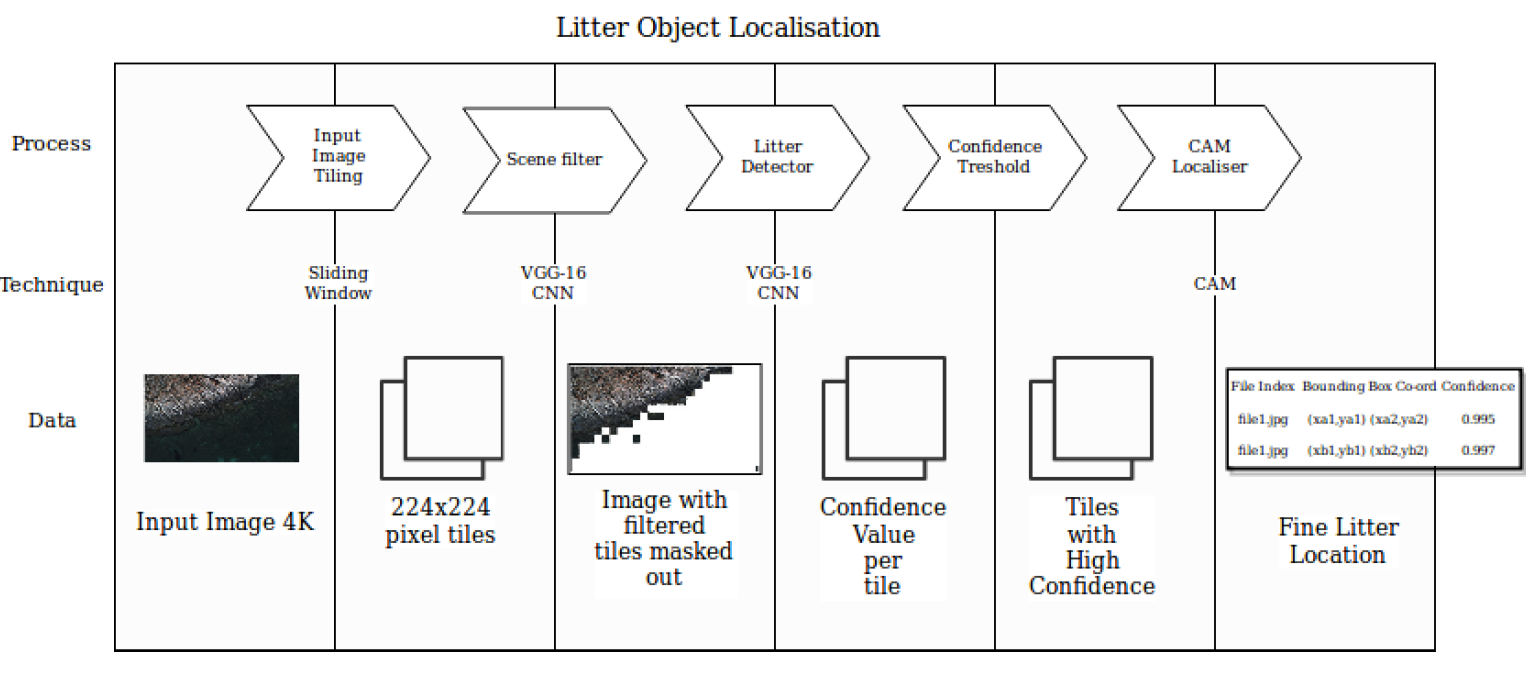
\includegraphics[width=0.9\linewidth]{small_litter_detection.png}
    \caption{Data flow and process diagram of the litter detection algorithm. (Source: \cite{small_litter_detection})}
    \label{fig:smalllitterdetection}
\end{figure}

Due to the dataset’s foreground-to-background sample ratio of 1:20, a confidence threshold was used to refine the detection results. \gls{cam} was employed to improve the \gls{iou} score by highlighting relevant foreground areas. Thresholding and normalising the heatmap allowed for generating masks that effectively located the target objects. An \gls{iou} threshold of 0.01 for \gls{nms} was used to facilitate the detection of very small objects.
Furthermore, the study identified that stones and vegetation were among the classes frequently misclassified as litter. To address this issue, the authors proposed a two-stage model incorporating a terrain filter to automate the detection of misclassifications, which provided improved results. They also concluded that litter with more defined shapes was easier to detect for both human annotation and algorithmic detection. 
Finally, the authors also trained the Faster \gls{rcnn} detection model on the same dataset and observed lower performance metrics, which were attributed to its inability in handling highly variable background representations \cite{small_litter_detection}.

\subsection{TACO: Trash Annotations in Context for Litter Detection}
\label{subsec:3_tacodataset}

Detecting litter in natural environments presents considerable challenges due to the variability of litter, which can be deformable, transparent, aged, fragmented, occluded, and camouflaged. Furthermore, models must contend with the wide variety of features found in natural landscapes. To tackle these issues, Proença and Simões introduced the \gls{taco} dataset in 2020 \cite{taco2020}. This dataset was created to feature images captured from a variety of global environments, as shown in Figure \ref{fig:taco1}, including beaches and urban areas, with litter segmented and annotated according to a hierarchical classification system \cite{taco2020}.

\begin{figure}[!htbp]
    \centering
    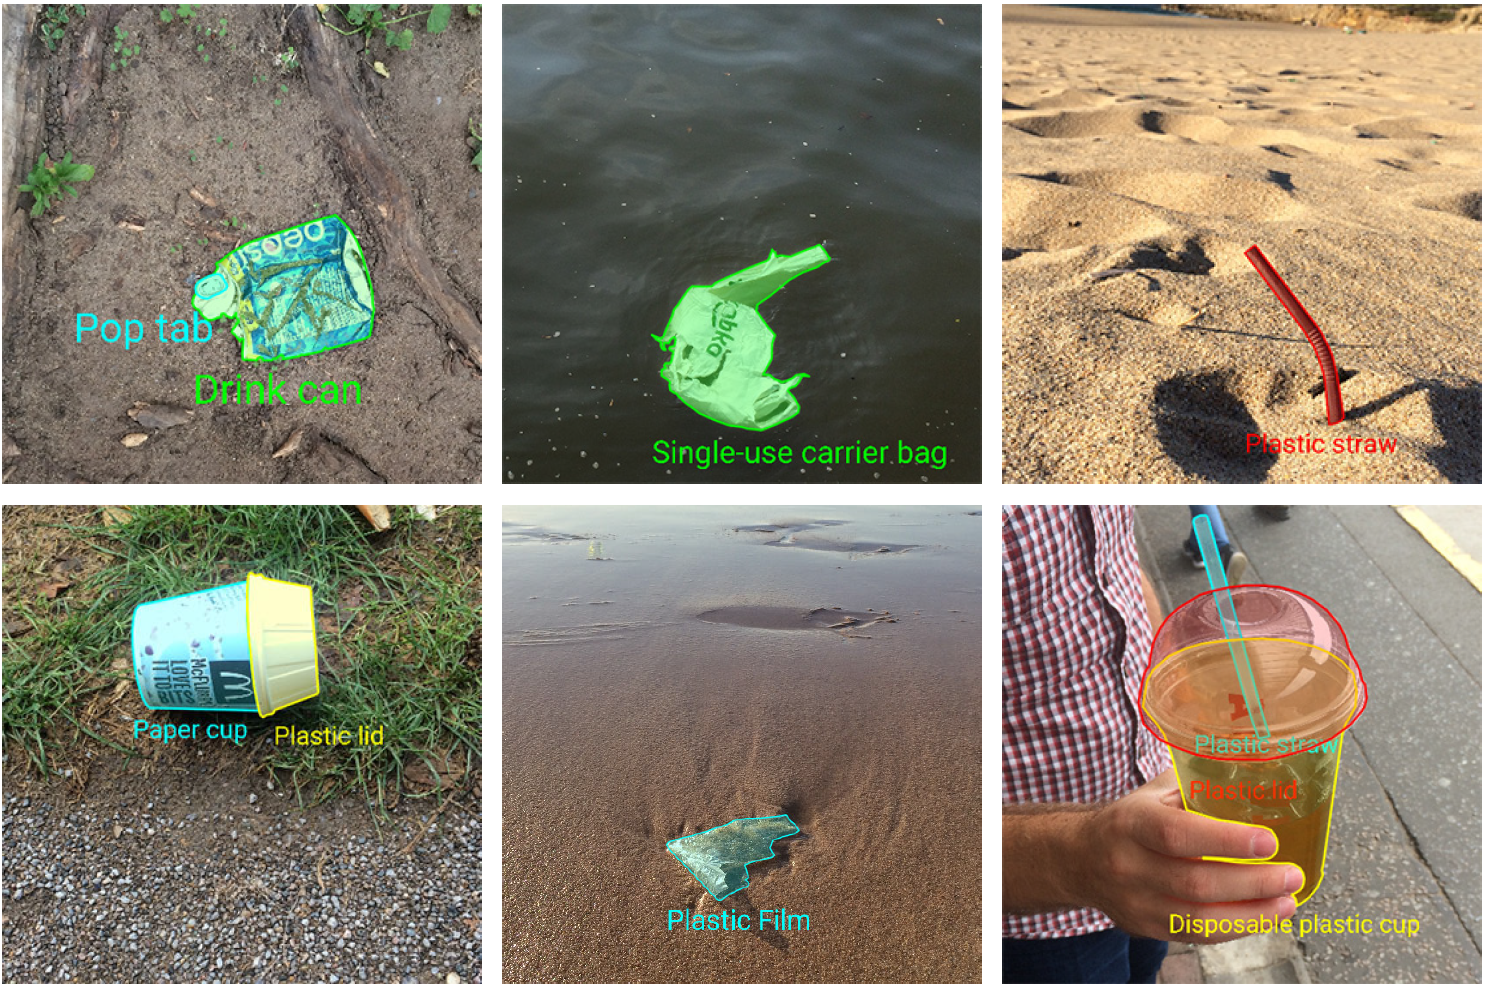
\includegraphics[width=0.8\linewidth]{taco1.png}
    \caption{Annotated images from the \gls{taco} dataset, with litter objects marked using polygon masks for instance segmentation. (Source: \cite{taco2020})}
    \label{fig:taco1}
\end{figure}

The \gls{taco} dataset includes 60 distinct litter categories, organised into 28 top-level (super) categories, as observed in Figure \ref{fig:taco2}. Unlike \gls{uav}-based datasets, \gls{taco} consists of images captured from ground-level natural environments. At the time of release, the dataset comprised 1,500 annotated images and 4,784 instances of litter, with an additional 3,918 new images currently awaiting annotation. The dataset uses polygon masks for annotation in an attempt to tackle the problem of both object detection, and instance segmentation \cite{taco2020}.
The authors conducted several experiments using Mask \gls{rcnn} to evaluate the dataset's performance. Two configurations were tested:
\begin{itemize}
    \item \textbf{\gls{taco}-1:} Identifying a single class of litter.
    \item \textbf{\gls{taco}-10:} Identifying ten distinct litter classes.
\end{itemize}

\begin{figure}[ht]
    \centering
    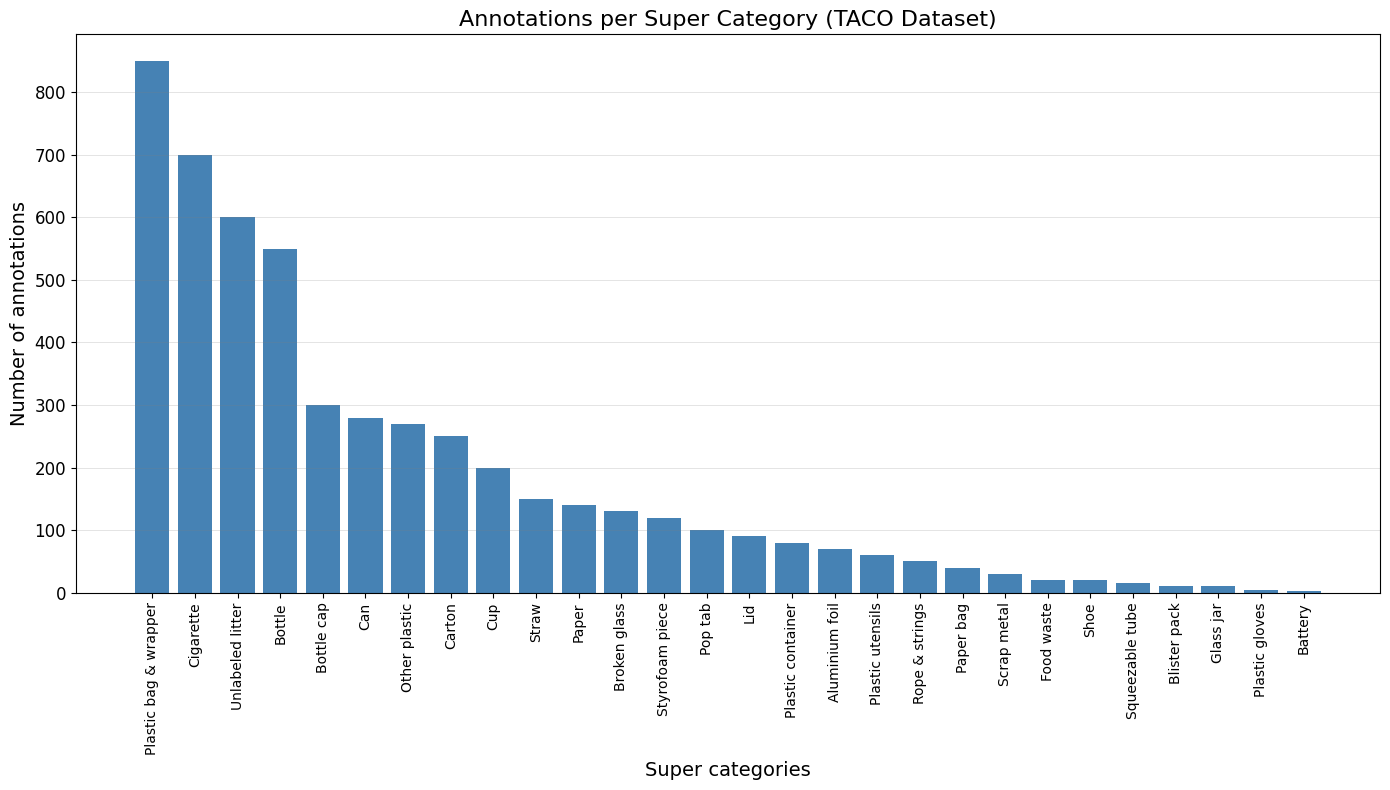
\includegraphics[width=1\linewidth]{taco2.png}
    \caption{Number of annotations per super category in the published version of the \gls{taco} dataset. (Source: \cite{taco2020})}
    \label{fig:taco2}
\end{figure}

The authors noted that the detection performance was notably low due to challenges in detecting small items, particularly cigarette butts, which led to a high rate of false positives and negatives. This was attributed to their small size, with most images resized to $1024 \times 1024$ pixels, causing many small objects (less than $20 \times 20$ pixels) to be missed. Larger objects, such as cans and bottles, were detected more accurately, though a considerable number of bottles were misclassified as cans. Confusion was also observed between \textit{plastic bags} and \textit{other litter}, which is understandable given the material similarities between these categories \cite{taco2020}.

\subsection{Multi-Level Approach to Waste Object Segmentation}
\label{subsec:3_mju-waste}

In 2020, Wang et al. also sought to address the challenge of waste object segmentation through a multi-level approach \cite{mju_waste}. To create their dataset, the authors collected waste items from a university campus, photographed individuals holding these items, and then annotated the images. The MJU-Waste dataset focuses solely on a single category, classifying all items under the label of \textit{waste}. The MJU-Waste dataset contains 2,475 annotated images and 2,525 instances of litter, all of which are annotated using polygon masks.
Unlike \gls{uav}-based datasets, the MJU-Waste dataset consists of images captured from controlled environments. The dataset includes segmentation masks, along with both raw and processed depth maps for all litter instances, captured using a Microsoft Kinect RGBD camera. However, due to sensor limitations, the depth frames contain missing values, particularly at reflective surfaces, occlusion boundaries, and distant regions. To address this, a median filter was applied to fill in the missing data and ensure the depth images were of high quality. Each image in the dataset was annotated with pixel-wise masks of the waste objects, and examples of colour frames, ground-truth annotations, and depth frames are provided in Figure \ref{fig:mjuwaste}. Alongside the semantic segmentation ground truths, object instance masks are also available \cite{mju_waste}.

\begin{figure}[!htbp]
    \centering
    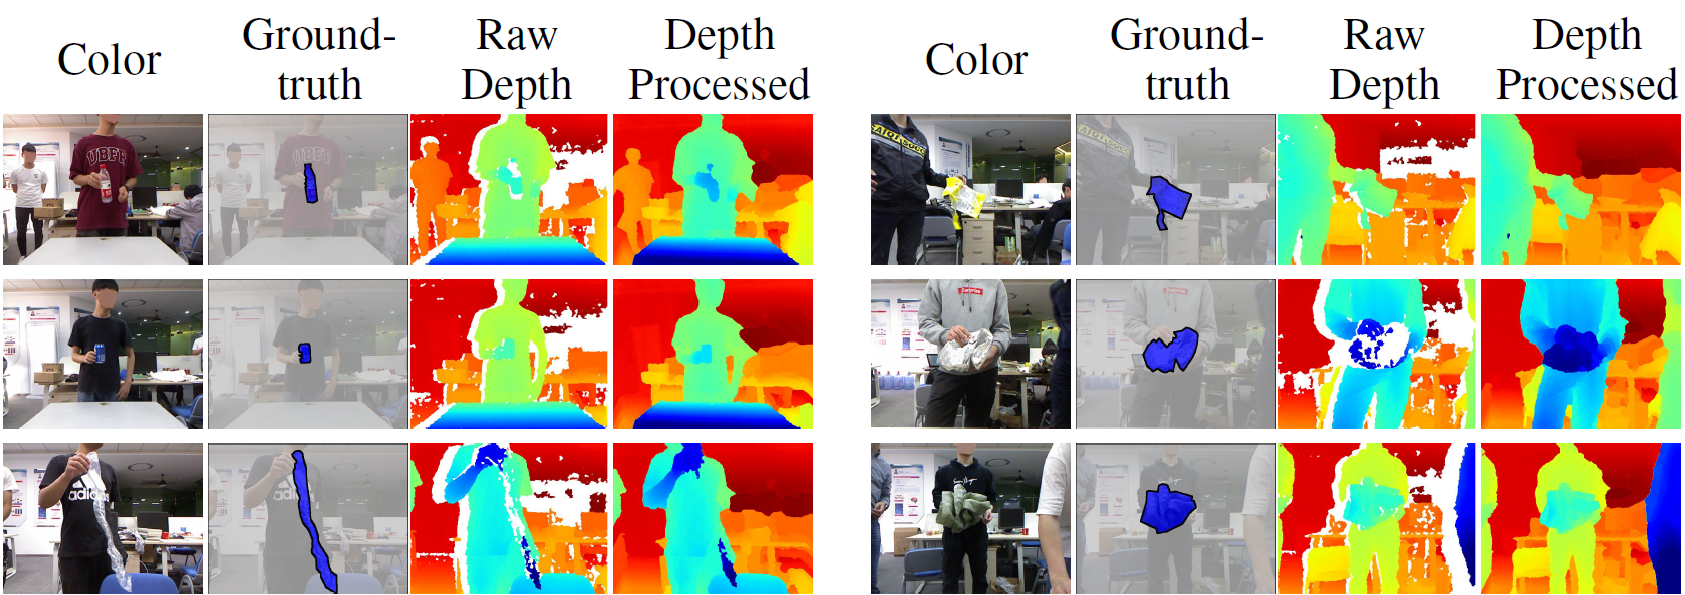
\includegraphics[width=1\linewidth]{mjuwaste.png}
    \caption{Sample RGB images, ground-truth annotations, and depth frames from the MJU-Waste dataset. (Source: \cite{mju_waste})}
    \label{fig:mjuwaste}
\end{figure}

The authors evaluate their proposed method against state-of-the-art semantic segmentation baselines. Their approach adopts a multi-level strategy for waste object segmentation, involving three key stages: first, scene-level parsing for initial coarse segmentation; second, object-level parsing to refine object region proposals; and third, pixel-level refinement using colour, depth, and spatial affinities. By combining inference from all three levels, the method achieves a coherent and accurate final segmentation.
In addition, the study focuses on two particularly challenging scenarios for waste object localisation: the hand-held setting, which is crucial for applications such as service robot interactions and smart trash bins, and waste objects found in natural environments. A significant challenge noted by the authors in both cases is the extreme variation in object scale, which leads to suboptimal performance from standard segmentation algorithms \cite{mju_waste}.
In comparison to the \gls{taco} dataset, the MJU-Waste dataset is split as follows: 60\% for training, 10\% for validation, and 30\% for testing. The evaluation metrics used include \gls{iou}, mean \gls{iou}, and pixel precision. The models tested include FCN-8s \cite{fcn}, PSPNet \cite{pspnet}, CCNet \cite{ccnet}, and DeepLabv3 \cite{deeplabv3}. Among these, DeepLabv3 performed best in terms of \gls{iou} and mIoU, while CCNet excelled in pixel precision. Notably, DeepLabv3 also outperformed other models when tested on the \gls{taco} dataset.
The authors also conclude that their multi-level approach proved effective, with scene-level segmentation, object-level segmentation, and pixel-level refinement working together to produce high-quality localisation results \cite{mju_waste}.

\subsection{UAVVaste: Vision-Based Trash and Litter Detection in Low Altitude Aerial Images}
\label{subsec:3_uavvaste}

In 2021, Kraft et al. addressed the challenge of detecting litter and the associated issue of mapping detected litter geographically \cite{uavvaste}. Their proposed system employed a \gls{uav} equipped with onboard sensors to process low-altitude aerial imagery. A key feature of the system was its reliance on low-cost, commercially available components, which were integrated into a self-contained solution capable of autonomous operation during \gls{uav} patrol missions.
A notable contribution of their research was the introduction of an application-specific dataset, UAVVaste. This dataset consists of 772 images with 3,716 bounding box annotations, as illustrated in Figure \ref{fig:uavvaste1}, and is dedicated to a single category: litter, labelled as \textit{rubbish}. The creation of this dataset was motivated by the lack of domain-specific data tailored to \gls{uav}-based litter detection. Compared to the \gls{taco} dataset, the UAVVaste dataset features a marked distribution shift, characterised by smaller object sizes, reflecting the unique challenges of detecting litter in aerial imagery \cite{uavvaste}.

\begin{figure}[!htbp]
    \centering
    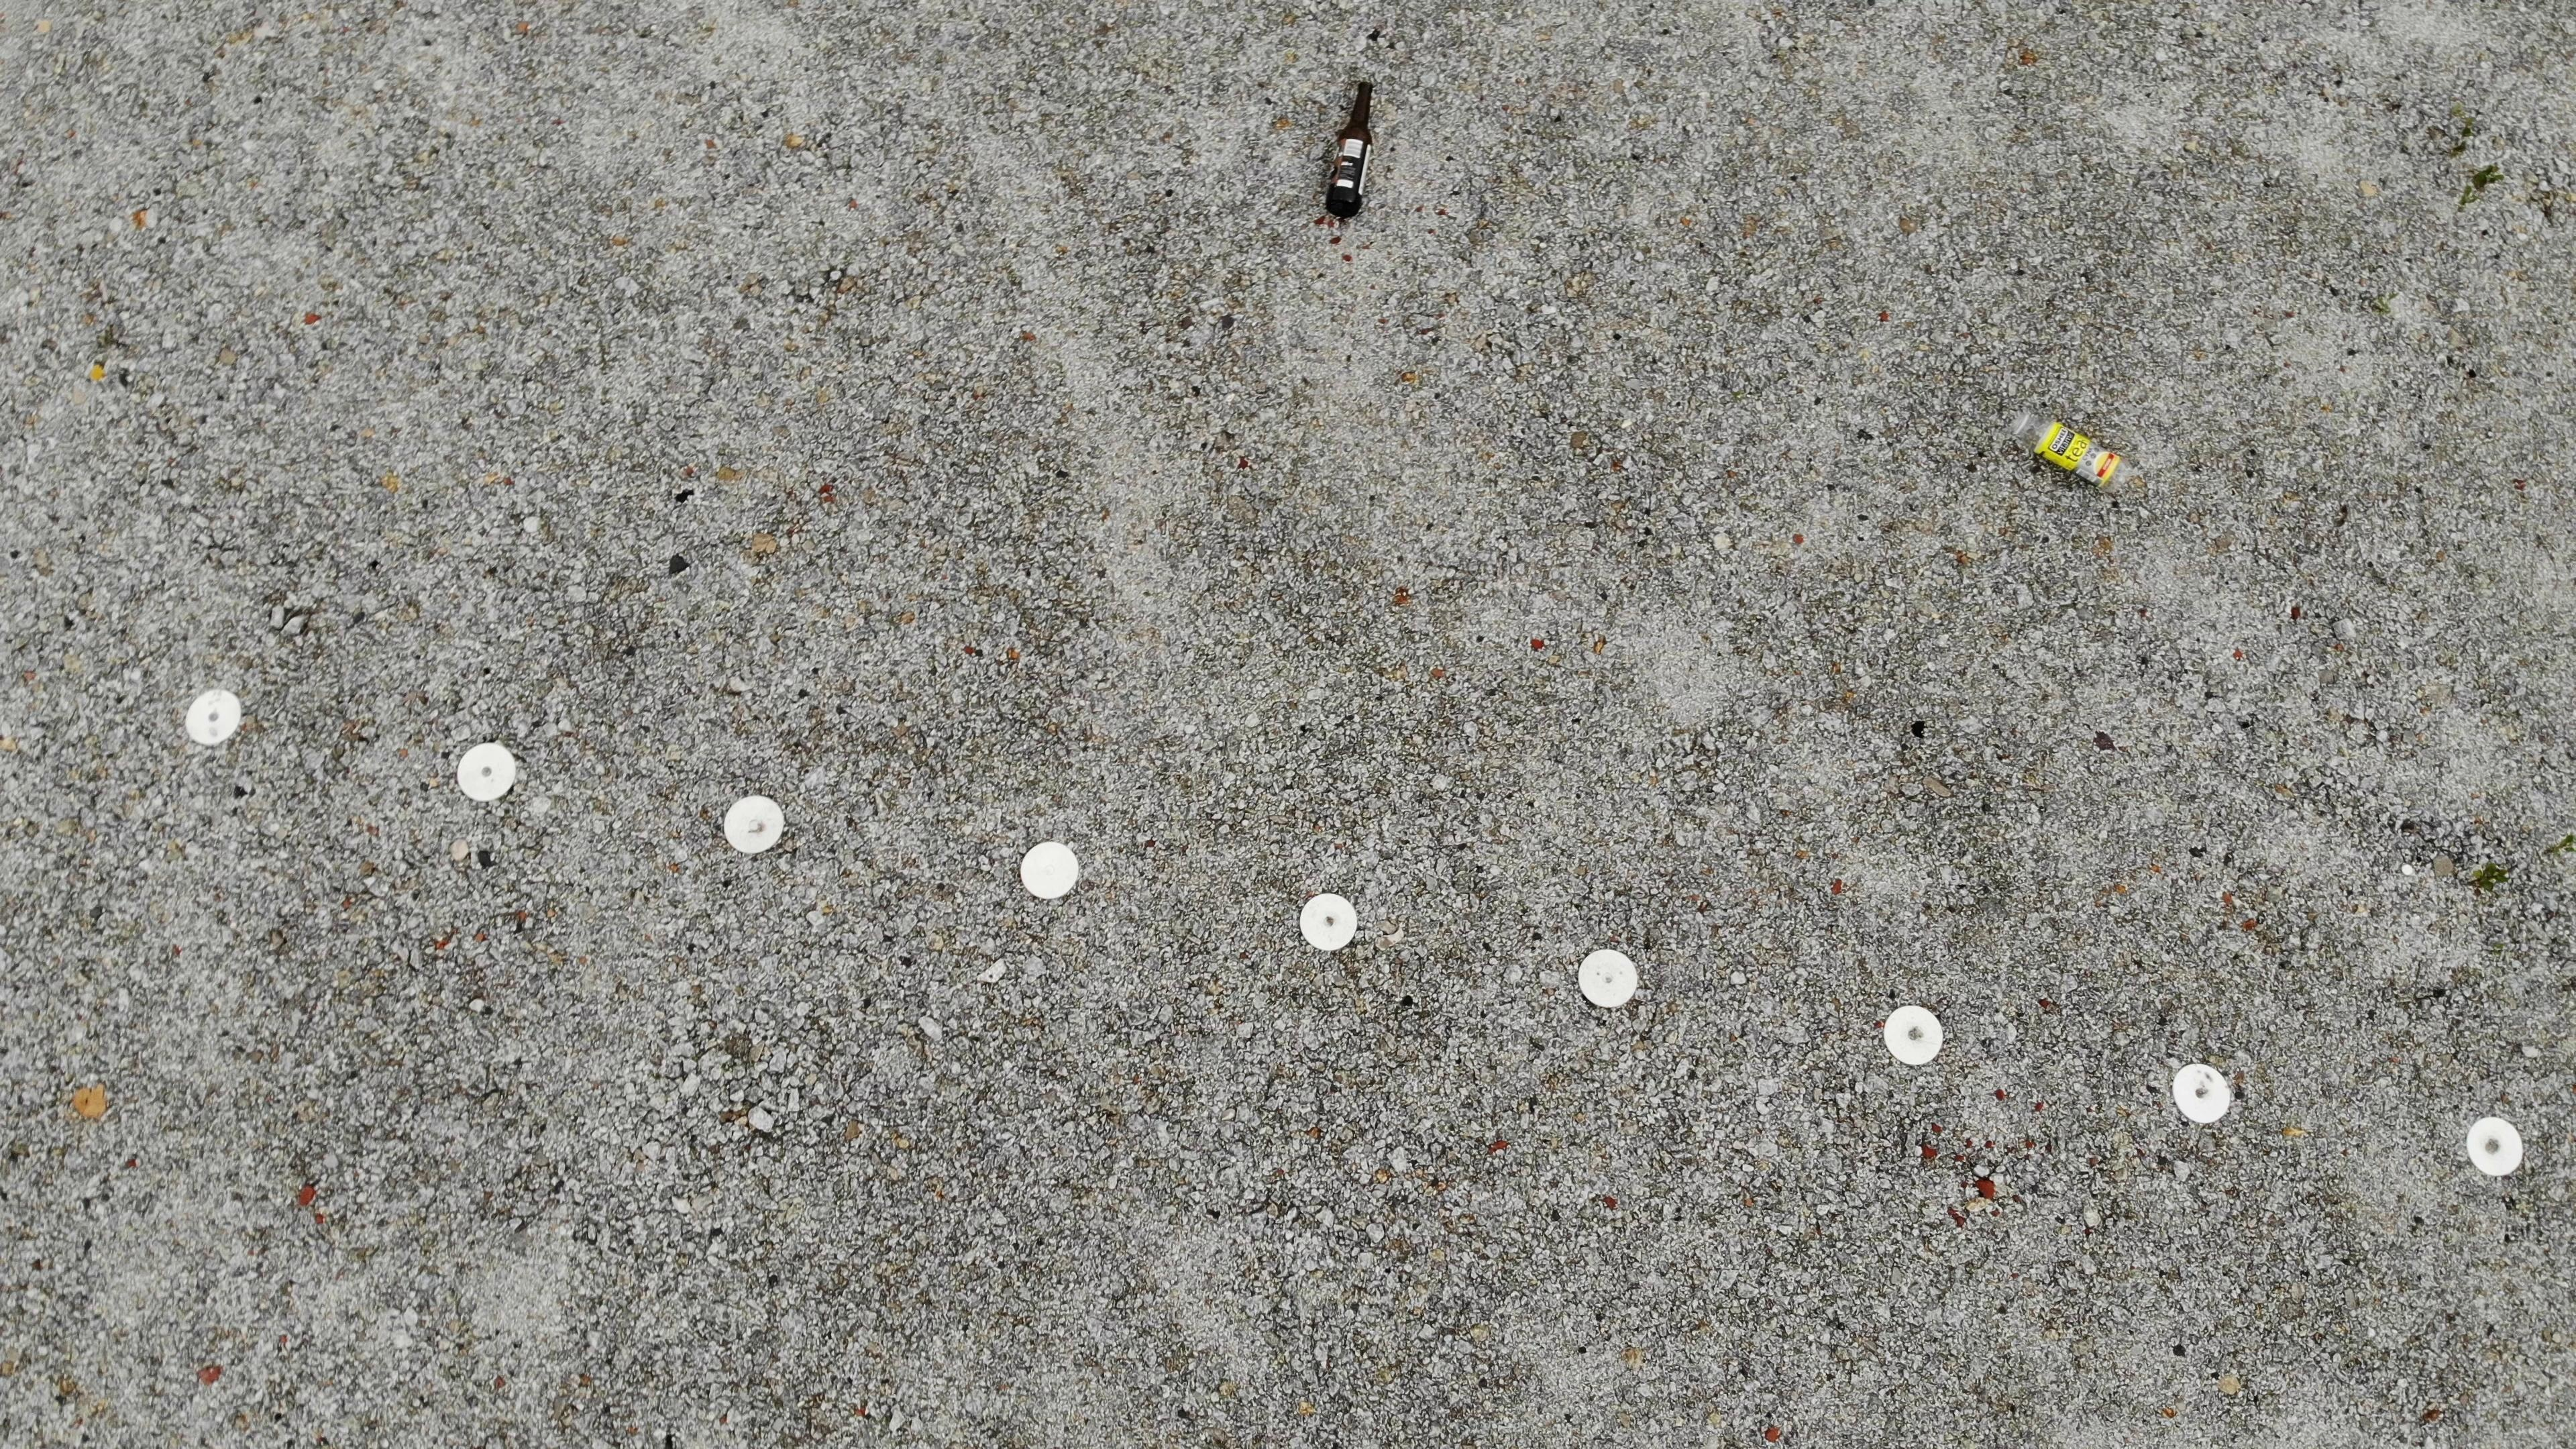
\includegraphics[width=0.9\linewidth]{uavvaste1.png}
    \caption{Sample images from the UAVVaste dataset with litter objects annotated using bounding boxes. (Source: \cite{uavvaste})}
    \label{fig:uavvaste1}
\end{figure}

The \gls{uav} hardware used in the study included a Pixhawk 2 autopilot controller, a Here2 \gls{gps}/\gls{gnss} module equipped with a barometric pressure sensor, and a downward-facing camera stabilised using a gimbal. The computational platform featured multiple components, including an Nvidia Xavier NX, a Google Coral USB (\gls{tpu}), and a Raspberry Pi 4. A variety of neural network architectures were evaluated for litter detection. These included \gls{ssd} detectors with lightweight backends optimised for TensorFlow Lite, which operated efficiently on the Google Coral \gls{tpu}, as well as \gls{yolo}v3 and \gls{yolo}v4 and their lightweight variants. For models deployed on the Nvidia Xavier NX, TensorRT was utilised to optimise performance. Additionally, EfficientDet with a MobileNet backend was implemented. Training these models involved transfer learning, leveraging pre-trained weights from the \gls{coco} dataset to improve performance \cite{uavvaste}.

% \begin{figure}[!htbp]
%     \centering
%     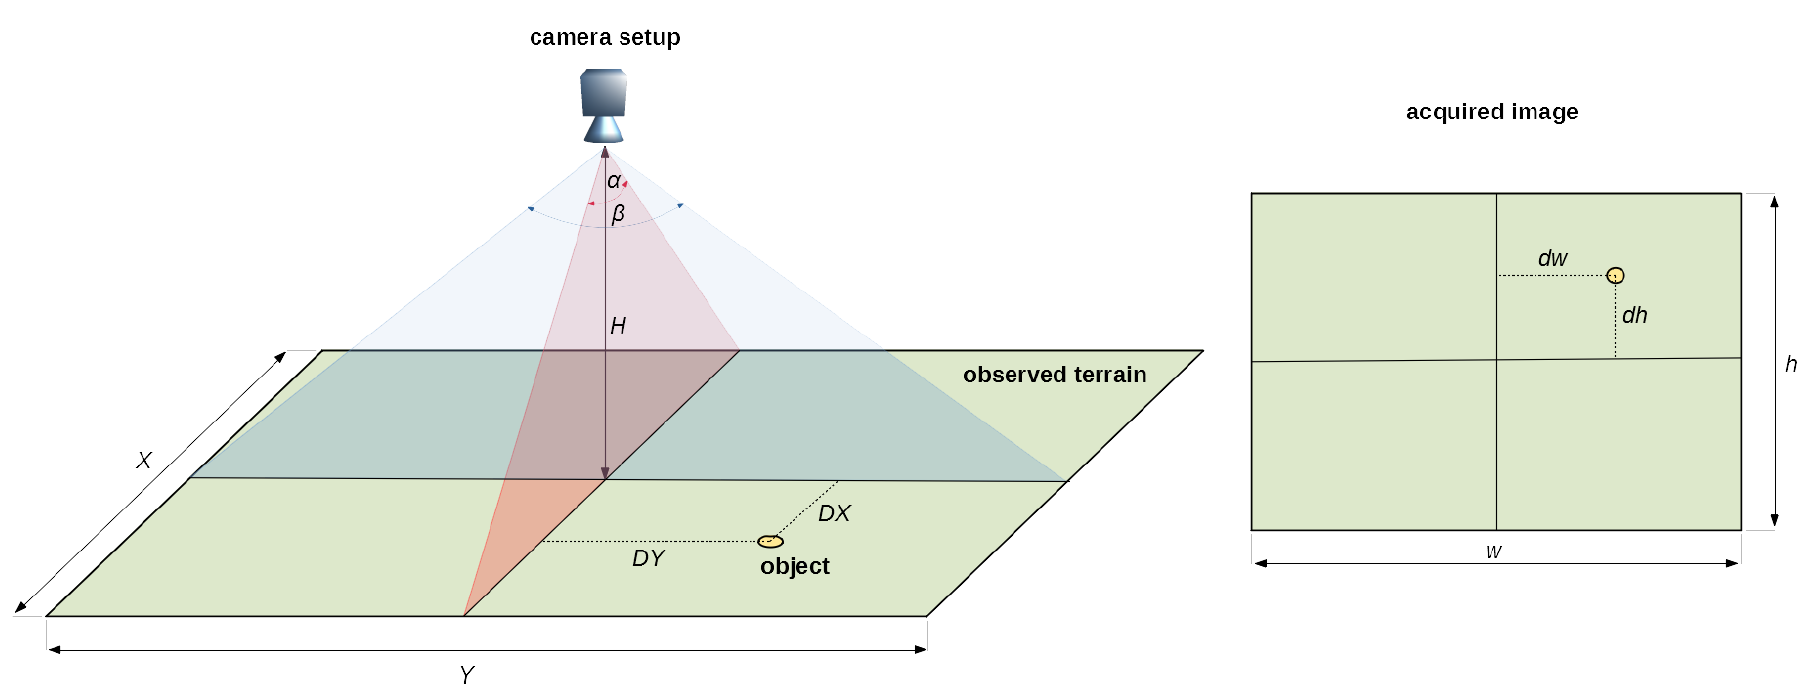
\includegraphics[width=0.9\linewidth]{uavvaste2.png}
%     \caption{A schematic representation of the camera setup and acquired image, along with the key parameters. (Source: \cite{uavvaste})}
%     \label{fig:uavvaste2}
% \end{figure}

% A significant portion of the study focused on creating a geolocation algorithm, which marks detected litter objects on a map using the UAV’s onboard sensors. This process required camera calibration, performed using the Kalibr library, and lens distortion correction, ensuring accurate geometric relationships between the image and real-world coordinates. The algorithm assumed a vertical downward orientation for the camera during operation. Using the known viewing angles of the camera and the UAV’s altitude, the algorithm calculated the size of the area captured in each image. Figure \ref{fig:uavvaste2} provides a schematic representation of the camera setup and the acquired image, highlighting the key parameters involved in the process. While the camera parameters were determined with high precision, the accuracy of object localisation on the map was predominantly influenced by the accuracy of altitude measurements. The authors observed that any error in altitude measurement would proportionally affect the localisation accuracy.
A significant portion of this study also involved developing a geolocation algorithm to map detected litter using \gls{uav} sensor data. Camera calibration and distortion correction were performed to ensure accurate mapping, assuming the camera faced directly downward. The algorithm used the \gls{uav}'s altitude and camera angles to estimate ground coverage, with localisation accuracy largely dependent on altitude measurement precision.
Alongside this spatial mapping component, model performance was evaluated using standard detection metrics. The evaluation included the \gls{map} scores from the \gls{coco} dataset, calculated at \gls{iou} thresholds of 0.5 and 0.95. Separate \gls{map} and recall scores were also reported for small, medium, and large objects. Among the models tested, \gls{yolo}v4 achieved the highest \gls{map}, while EfficientDet excelled in recall, particularly for smaller objects \cite{uavvaste}.

\subsection{ZeroWaste: Towards Automated Waste Recycling}
\label{subsec:3_zerowaste}

In 2022, Bashkirova et al. introduced the first industrial-grade, in-the-wild waste detection and segmentation dataset, ZeroWaste, making a significant contribution to computer-aided waste detection \cite{zerowaste}. The dataset features four categories of litter: \textit{cardboard}, \textit{soft plastic}, \textit{rigid plastic}, and \textit{metal}. Unlike \gls{uav}-based datasets, the images in ZeroWaste were captured in real-world settings.
The ZeroWaste dataset includes 10,715 annotated images, collected from a high-quality paper conveyor at a single-stream recycling facility in Massachusetts, containing 27,744 instances of litter, all annotated in polygon format, as illustrated in Figure \ref{fig:zerowaste}. Data augmentation was also applied to the dataset to improve model generalisation by artificially increasing the variety of training samples. Furthermore, this four-class labelled dataset captures various waste items identified during the sorting process at the facility, which aims to separate high-quality paper from contaminants such as metal, plastic, brown paper, and cardboard \cite{zerowaste}.

\begin{figure}[!htbp]
    \centering
    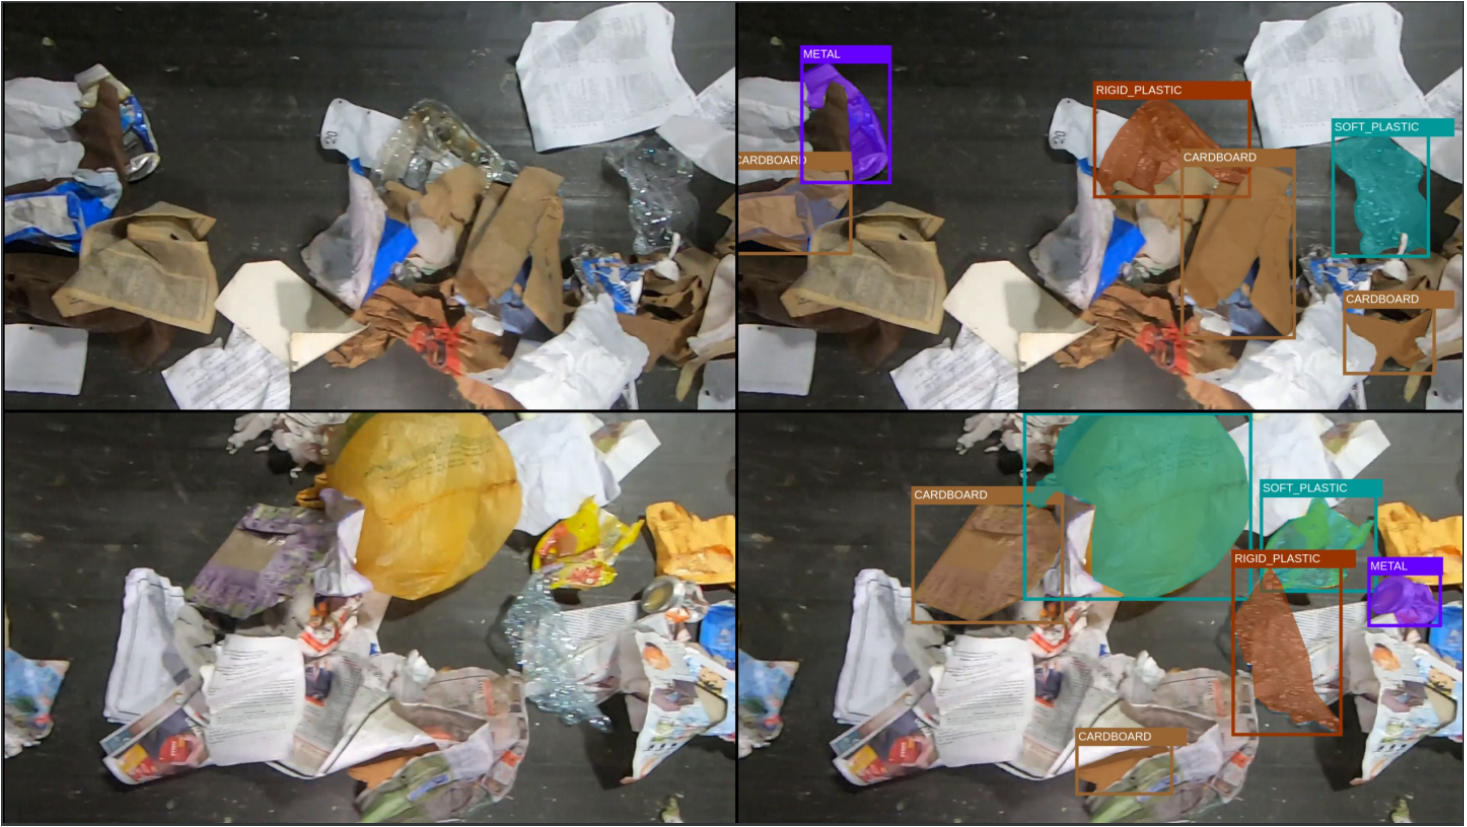
\includegraphics[width=0.9\linewidth]{zerowaste.png}
    \caption{Sample images (left) and ground truth polygon annotations (right) in the ZeroWaste dataset. (Source: \cite{zerowaste})}
    \label{fig:zerowaste}
\end{figure}

The data was gathered using two compact recording systems placed at the start and end of the conveyor belt during the facility's routine operations. The footage consists of 12 video sequences with a total duration of 95 minutes and 14 seconds, recorded at a frame rate of 120 \gls{fps} and a resolution of $1920 \times 1080$. To ensure high-quality data, the footage was processed to correct optical distortions, crop unnecessary elements, and remove motion blur.
The ZeroWaste dataset was divided as follows: 65\% for training, 15\% for validation, and 20\% for testing. The evaluation metrics used include \gls{ap} and \gls{map} at various thresholds, \gls{iou}, and pixel precision. The models tested include RetinaNet, Mask \gls{rcnn}, TridentNet \cite{tridentnet}, and DeepLabv3, and a series of experiments were conducted, including fully, semi, and weakly supervised learning.
The results revealed that the ZeroWaste dataset posed considerable challenges for state-of-the-art detectors such as Mask \gls{rcnn}. However, TridentNet emerged as the top-performing detector, while DeepLabv3 achieved the best results in terms of segmentation \cite{zerowaste}.

\subsection{PlastOPol: Litter Detection with Deep Learning}
\label{subsec:3_plastopol}

To address the issue of litter accumulation, Córdova et al. investigated the efficacy of lightweight neural networks for detecting litter in real-world environments with complex and crowded image backgrounds \cite{plastopol}. The study also evaluated the feasibility of deploying these models on mobile devices with limited memory capacity. Their 2022 publication presented two key contributions: a comparative analysis of state-of-the-art deep learning techniques for image-based litter and waste detection and the introduction of a novel dataset, PlastOPol, comprising 2,418 images captured in real-world conditions with 5,300 litter annotations.
The PlastOPol dataset includes a single class, with all litter items categorised under the label \textit{litter}. The dataset consists of images from natural settings rather than being derived from \gls{uav} data. These images were sourced using the Marine Debris Tracker and are publicly available under a Creative Commons Attribution licence. The dataset was annotated in a bounding box format and focused on the problem of object detection. Of the 5,300 annotated instances, 90.98\% are large objects, 8.40\% are medium objects, and only 0.62\% are small objects \cite{plastopol}.

\begin{figure}[!htbp]
    \centering
    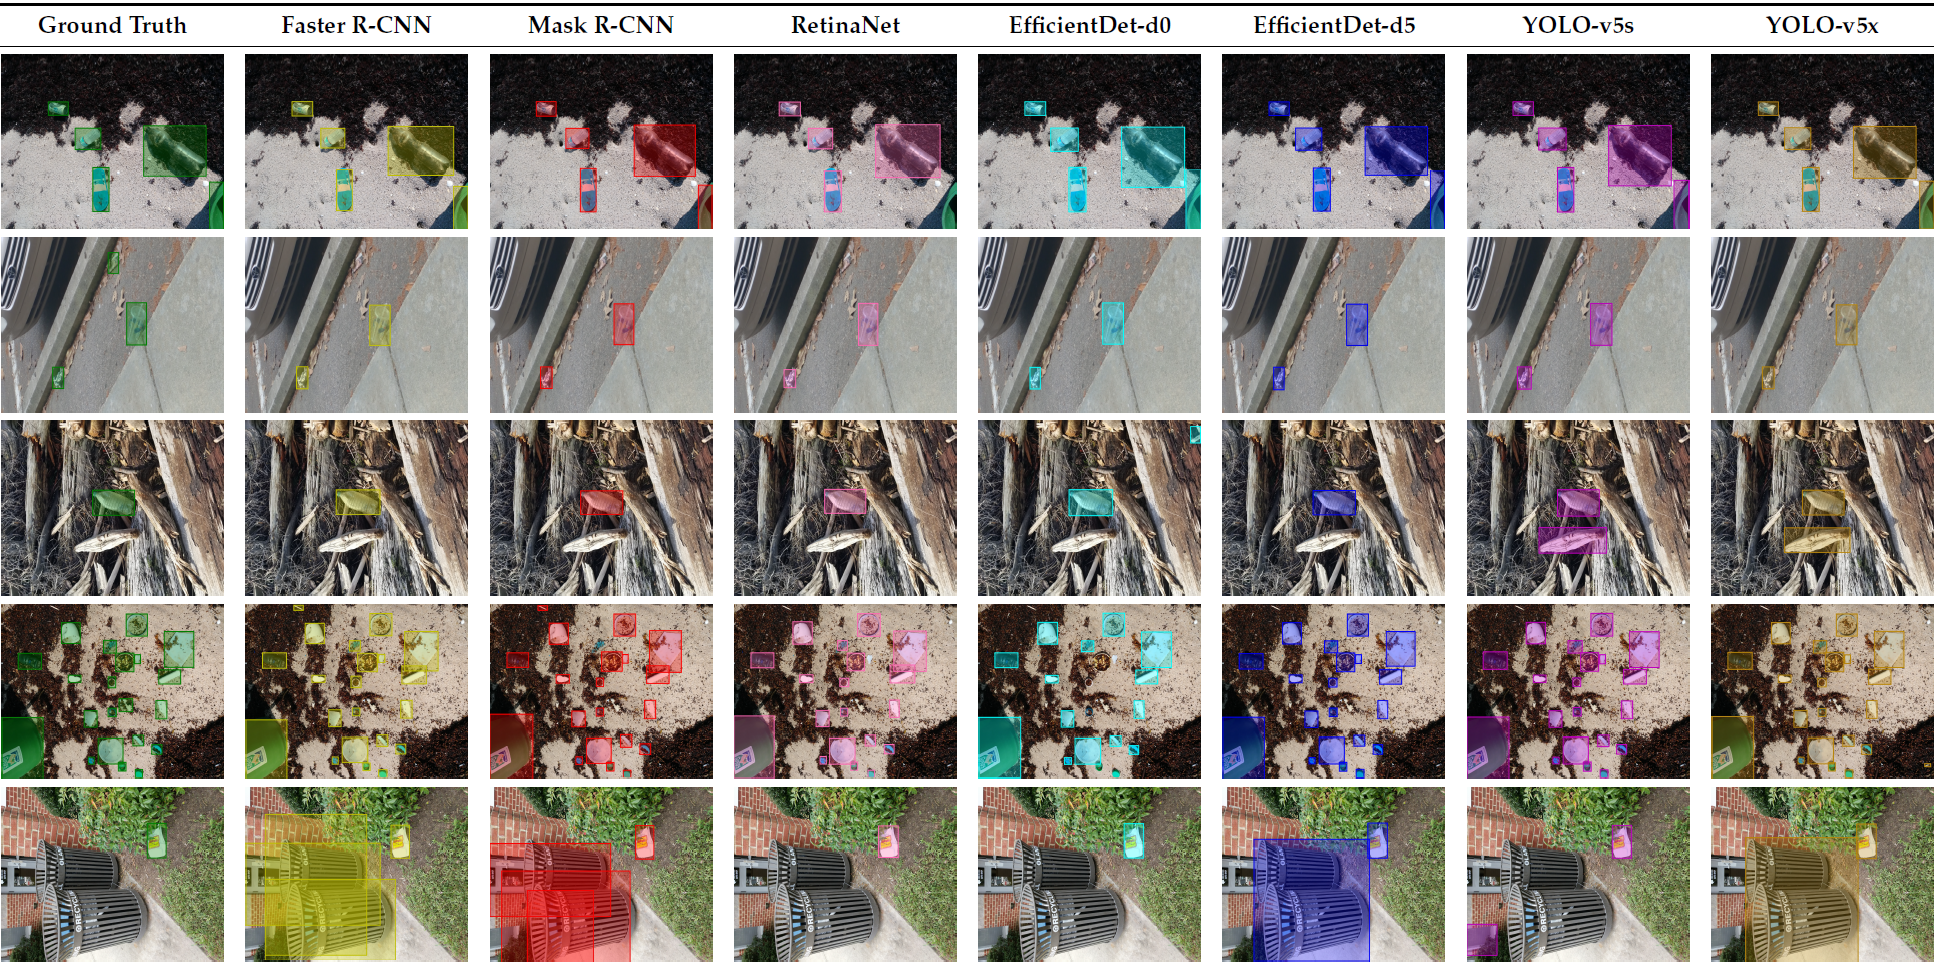
\includegraphics[width=1\linewidth]{plastopol.png}
    \caption{Visual detection results on the PlastOPol dataset. (Source: \cite{plastopol})}
    \label{fig:plastopol}
\end{figure}

To assess the performance of various deep learning models in detecting litter, the authors used both the proposed PlastOPol dataset and the publicly available \gls{taco} dataset. For the PlastOPol dataset, the data was split into 80\% for training and 20\% for testing. Evaluation metrics included \gls{ap}, \gls{map} at \gls{iou} threshold 0.5, F1 score, and recall. The models tested included EfficientDet, Faster \gls{rcnn}, Mask \gls{rcnn}, RetinaNet, and \gls{yolo}v5. As shown in Figure \ref{fig:plastopol}, the visual detection results on the PlastOPol dataset highlight the performance of these models in identifying litter objects across different environments.
The experiment results demonstrated that \gls{yolo}v5 was the best-performing model overall. The authors also observed that \gls{yolo}v5 and EfficientDet were the fastest models, even when deployed on mobile devices. However, they noted that all methods struggled with detecting small objects, such as cigarette butts. Notably, \gls{yolo}v5x outperformed Faster \gls{rcnn} and Mask \gls{rcnn} in terms of speed \cite{plastopol}.

\subsection{Real-Time UAV Trash Monitoring System}
\label{subsec:3_haida}

In 2022, Liao and Juang developed a marine litter detection system using \gls{uav}s \cite{haida}. Their goal was to reduce reliance on manual efforts and offer a more efficient method for identifying marine debris. The real-time \gls{uav} trash monitoring system consisted of nine components: \gls{uav}s, a message queuing system, a database, a video streaming server, a connector, a \gls{uav} control station, a web service, a \gls{uav} map, and a data analysis module, as illustrated in Figure \ref{fig:haida1}. The ground station incorporated key elements, such as the video streaming server, Kafka, the Kafka connector, MongoDB, and the web service. The system addressed two key challenges: object detection and geolocation, and as part of the system's development, the authors introduced the HAIDA dataset. This dataset, collected on the NTOU campus, was used to train the object detection model and contains two types of litter objects: \textit{garbage} and \textit{bottles}. The data was gathered using a \gls{uav} equipped with a Pixhawk controller and an NVIDIA Jetson Xavier NX. The UAV operated at altitudes ranging from 1 to 10 metres \gls{agl} \cite{haida}.

\begin{figure}[!htbp]
    \centering
    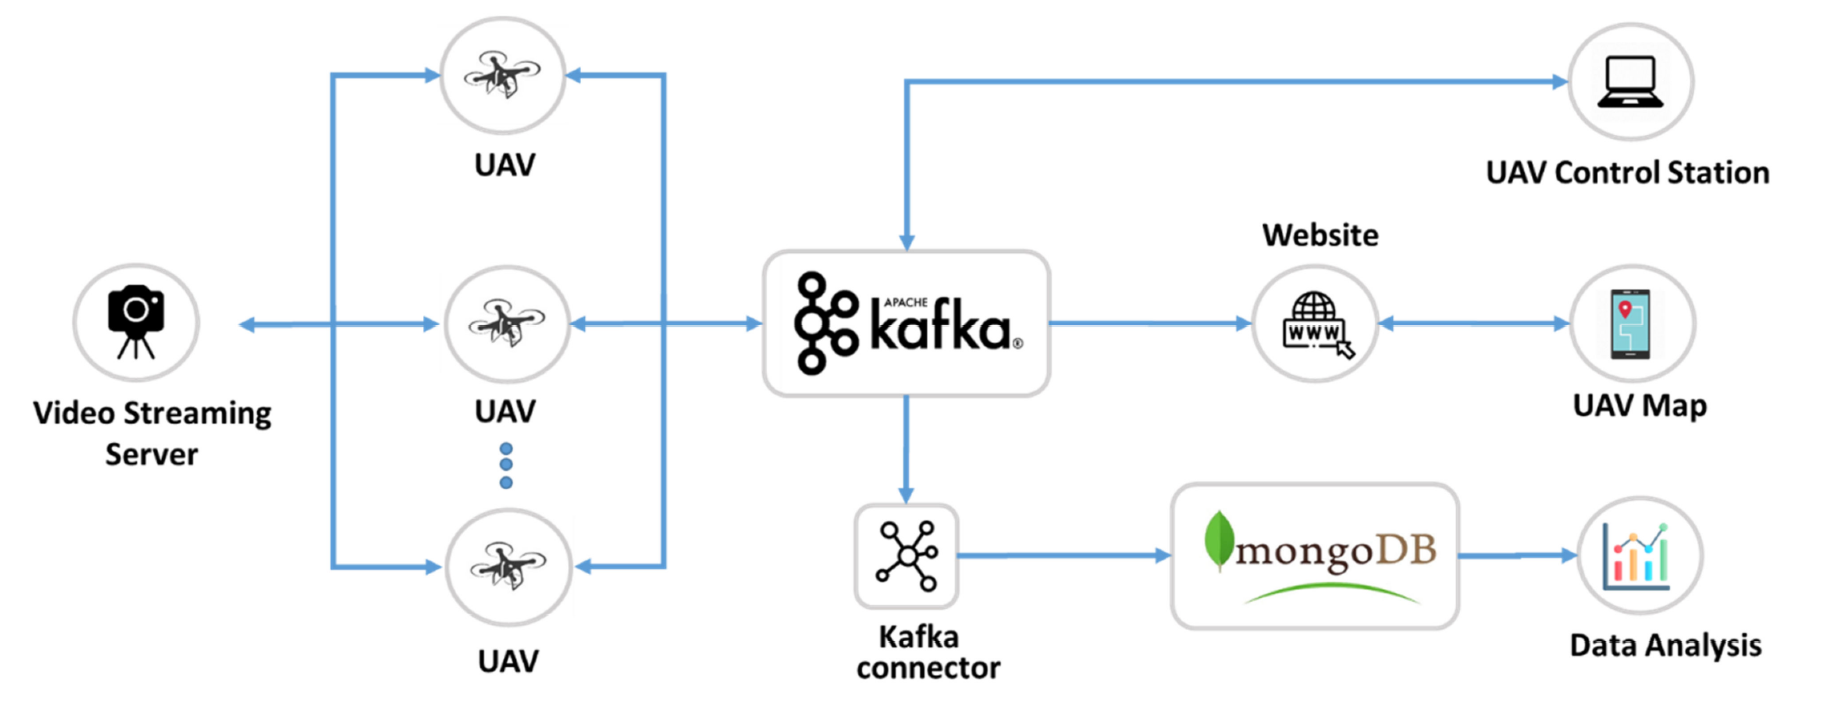
\includegraphics[width=0.7\linewidth]{haida1.png}
    \caption{The system architecture of the real-time \gls{uav} trash monitoring system. (Source: \cite{haida})}
    \label{fig:haida1}
\end{figure}

The HAIDA dataset comprises 1,319 annotated images, with 6,475 instances of litter, including 3,904 garbage objects and 2,571 bottle objects. Additionally, 456 images in the dataset contain no litter. The authors utilised the dataset to train the \gls{yolo} object detection model (version unspecified). The results showed that the model was able to identify trash objects with an \gls{ap} of over 70\% at a 0.5 \gls{iou} threshold. Notably, as shown in Figure \ref{fig:haida2}, the detection confidence for small objects was high, with confidence scores of 98.27\%, 64.65\%, and 91.86\% for different categories of litter.
The real-time \gls{uav} trash monitoring system operated by first collecting \gls{uav} footage as the drone flew across predetermined waypoints. The footage was then transmitted to a server via Kafka, where it was stored in an online database such as Oracle, MySQL, or MongoDB. Using this stored data, the server applied the trash detection model to identify litter both in the images and on a map. Control stations, both mobile and desktop, could make requests to the server to retrieve the map data, which displayed the locations of detected litter \cite{haida}.
To estimate litter geolocation, the authors followed an approach similar to that in \cite{uavvaste}, calculating pollution area based on \gls{uav} altitude, camera angles, and object size in the image. This enabled a reliable approximation of both the position and extent of detected waste \cite{haida}.

\begin{figure}[!htbp]
  \centering
  \begin{tabular}{cc}
    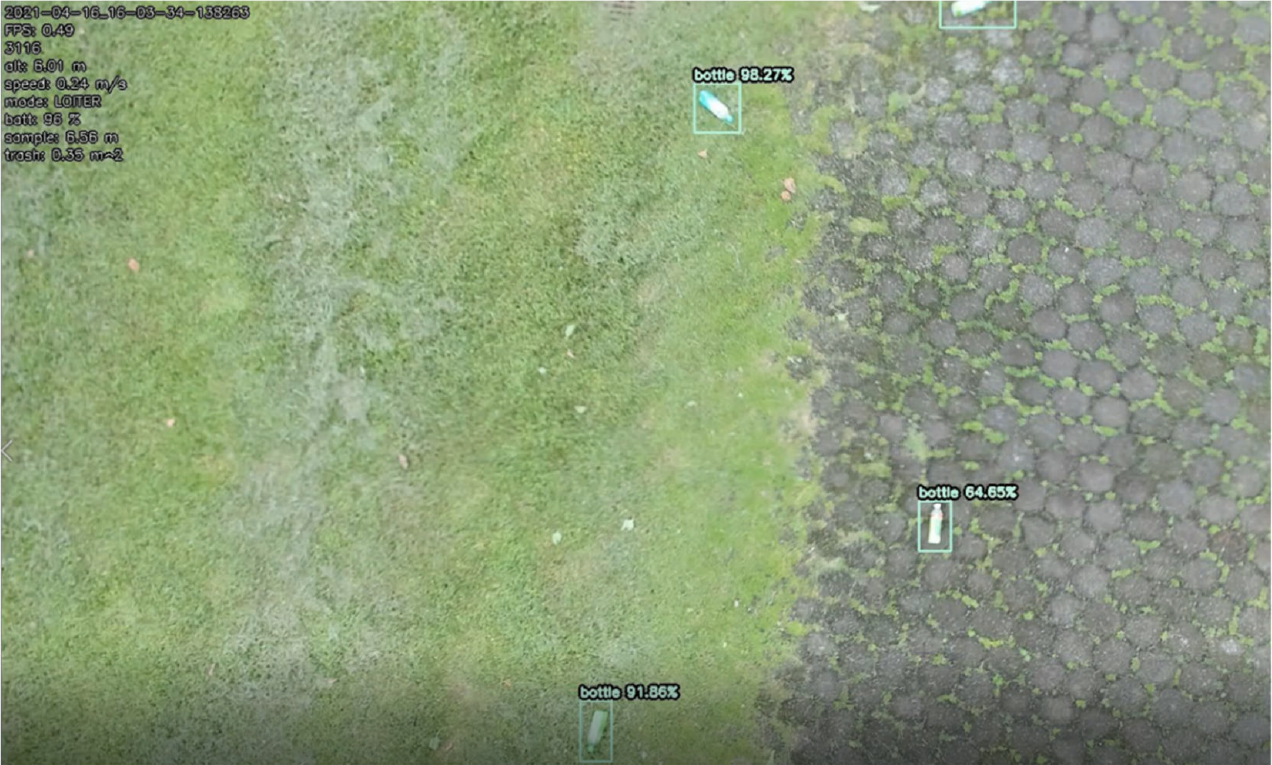
\includegraphics[width=0.48\textwidth, height=5cm]{haida2.png} &
    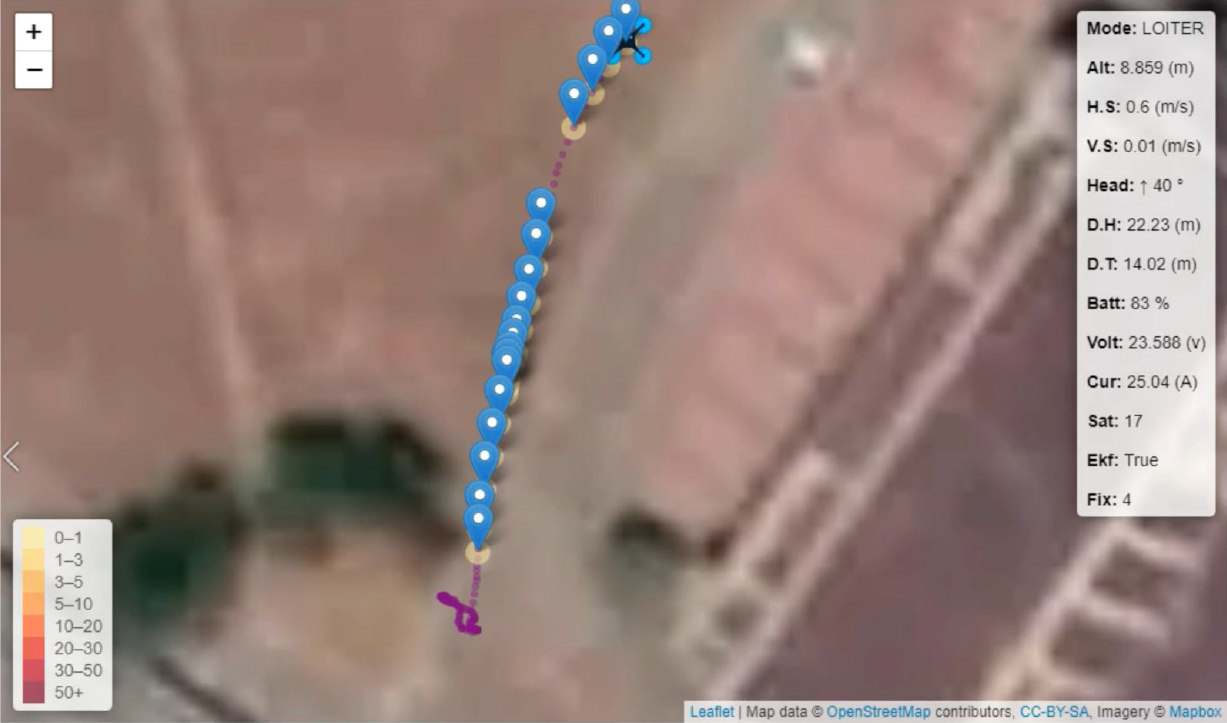
\includegraphics[width=0.48\textwidth, height=5cm]{haida3.png} \\
    \small (a) & \small (b) \\
  \end{tabular}\\
  \caption{\gls{uav} trash monitoring results on the NTOU campus. (a) Detection results from the UAV. (b) Detected litter plotted on a map, showing real-time monitoring and detection. (Source: \cite{haida})}
  \label{fig:haida2}
\end{figure}

% To tackle the problem of litter geolocation, the authors adapted a similar approach to the one described in \cite{uavvaste}, enabling the calculation of the detected trash pollution area based on several factors. These factors include the camera’s horizontal and vertical angle of view, the UAV’s altitude, the camera's field of view, the dimensions of the camera's image, the size of the detected trash in the image, and the detected trash's area in both the image and the real-world environment. By incorporating these variables, the system can accurately estimate the location and extent of trash pollution in the area \cite{haida}.

\subsection{Outdoor Trash Detection in Natural Environment}
\label{subsec:3_bangladeshi}

As populations in underdeveloped nations continue to grow, the challenges associated with trash production and disposal have become more urgent. Aware of the time-consuming and potentially hazardous nature of manual litter classification, Das et al. (2023) aimed to tackle this issue by developing automated methods for more efficient and safer waste management \cite{bangladeshi}. To achieve this, they focused on collecting data that accurately captured the complexities of litter in Bangladesh, creating an outdoor dataset, and incorporating OpenLitterMap to broaden its scope. This dataset comprises images from natural settings, not \gls{uav}-based data, and includes ten categories of litter: \textit{tissue paper}, \textit{plastic}, \textit{medical waste}, \textit{rope}, \textit{paper}, \textit{cigarette butts and boxes}, \textit{metal}, \textit{glass}, \textit{organic waste}, and \textit{textiles}. Initially consisting of 1,283 annotated images, the dataset was expanded to 4,418 by integrating data from OpenLitterMap, a global database containing litter and plastic images. The Bangladeshi dataset contains 6,178 instances of litter, which was extended to 8,077 while retaining the ten distinct classes \cite{bangladeshi}.

\begin{figure}[!htbp]
  \centering
  \begin{tabular}{c}
    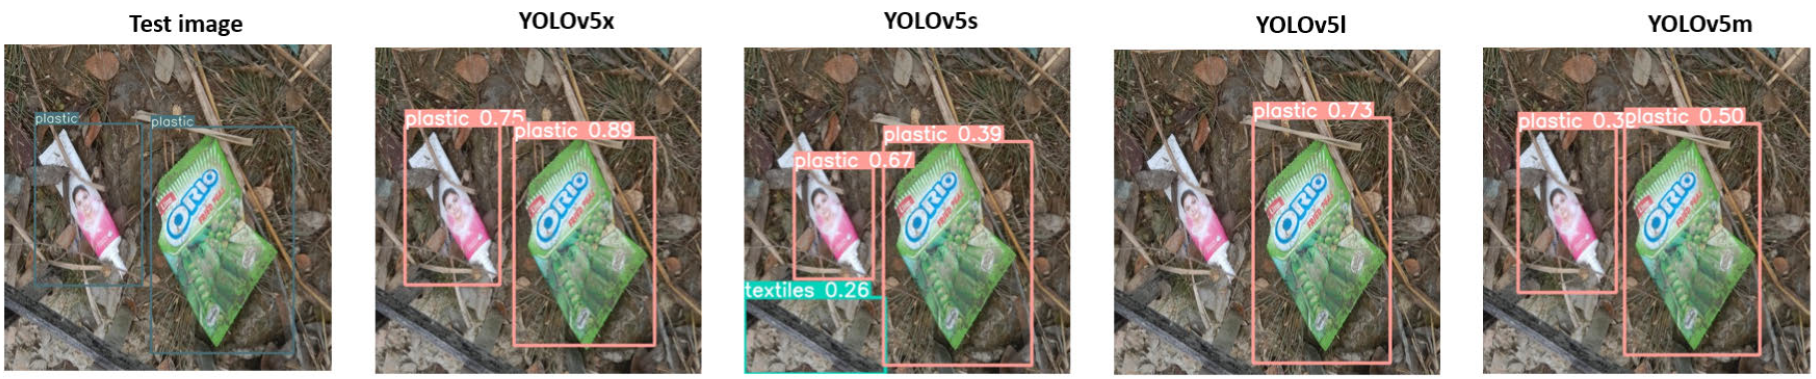
\includegraphics[width=1\textwidth]{bangladeshi1.png} \\
    \small (a)\\
    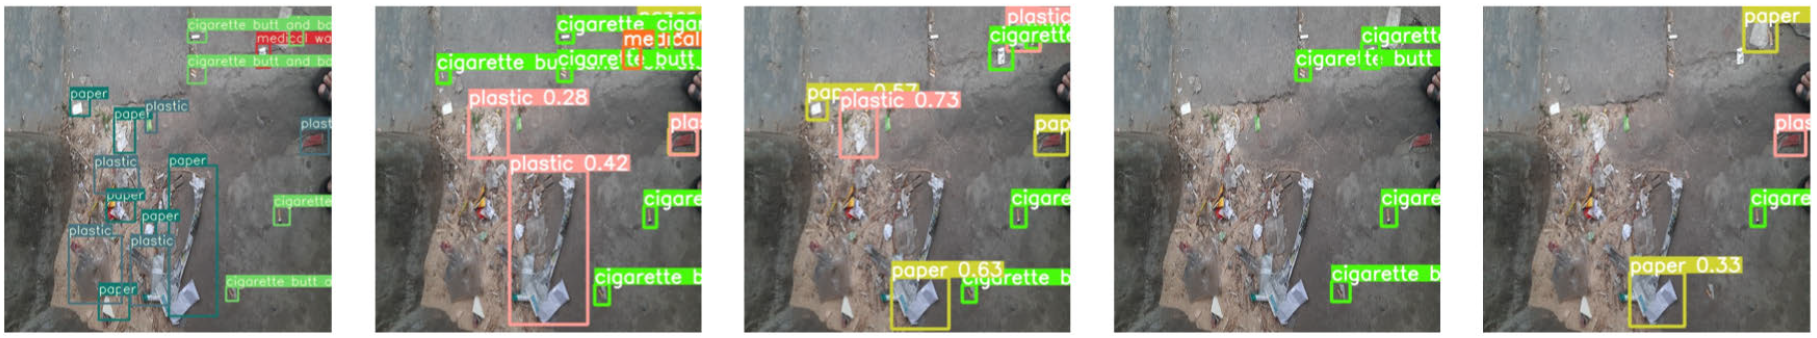
\includegraphics[width=1\textwidth]{bangladeshi2.png} \\
    \small (b) \\
  \end{tabular}\\
  \caption{Litter detection results using different versions of the \gls{yolo}v5 model on the Bangladeshi dataset. (a) 2 instances of litter; (b) 17 instances of litter. (Source: \cite{bangladeshi})}
  \label{fig:bangladeshi}
\end{figure}

The experimental setup used for this study involved a comparison with the \gls{taco} and PlastOPol datasets. The Bangladeshi dataset was divided as follows: 80\% for training, 10\% for validation, and 10\% for testing. The evaluation metrics included \gls{ap} and \gls{map} at \gls{iou} thresholds from 0.5 to 0.95, as well as F1 score and recall. Several models were tested, including different versions of \gls{yolo}v5, \gls{yolo}v6, \gls{yolo}v8, and Faster \gls{rcnn}. The authors also employed data augmentation techniques during training and optimised model performance by adjusting hyperparameters.
In their study, the authors reported that \gls{yolo}v5x was the best-performing model, as visually demonstrated in Figure \ref{fig:bangladeshi}, which shows a comparison of the detection bounding boxes on the images, demonstrating the improved \gls{map} for the expanded dataset. However, single-class detection experiments on the \gls{taco} and PlastOPol datasets yielded better results compared to the Bangladeshi dataset. Das et al. also highlighted that in future work, they plan to expand the dataset to include a broader range of categories, such as ocean waste, which is currently absent. Additionally, other object detection methods, such as \gls{ssd}, Mask \gls{rcnn}, and EfficientDet, could also be evaluated using their dataset \cite{bangladeshi}.

\subsection{Use of UAVs and Deep Learning for Beach Litter Monitoring}
\label{subsec:3_beach_litter}

In 2023, Pfeiffer et al. proposed a framework for an autonomous beach litter monitoring and retrieval system based on drone surveys and object detection using deep learning techniques \cite{beach_litter}. Their research combined drone footage collected from the islands of Malta and Gozo, Sicily (Italy), and the Red Sea coast with publicly available litter datasets, which were subsequently used to train an object detection model for identifying litter in the captured footage. Figure \ref{fig:beachlitter1} illustrates the overall framework of the proposed beach litter monitoring system. To address both object detection and geolocation challenges, the authors compiled a \gls{uav} dataset collected with DJI Phantom 4 Pro 2.0 and DJI Mavic 2 UAVs. The dataset covered altitudes ranging from 10 metres above ground level to 60 metres above sea level and included 67 types of litter, which were categorised into seven meta-classes: \textit{clothing \& fabric}, \textit{glass}, \textit{small objects}, \textit{metal litter}, \textit{paper \& cardboard}, \textit{plastic}, and \textit{other waste}.
Additionally, the collected Beach Litter Dataset contains 4,126 annotated images and 10,611 litter instances, including 1,154 images with no litter present. The dataset was divided as follows: 60\% for training, 20\% for validation, and 20\% for testing. The models were evaluated using metrics such as \gls{ap},\gls{map} (at 0.5–0.95), F1 score, and recall, with the \gls{yolo}v5 model being the primary model used for training \cite{beach_litter}. 

\begin{figure}[!htbp]
    \centering
    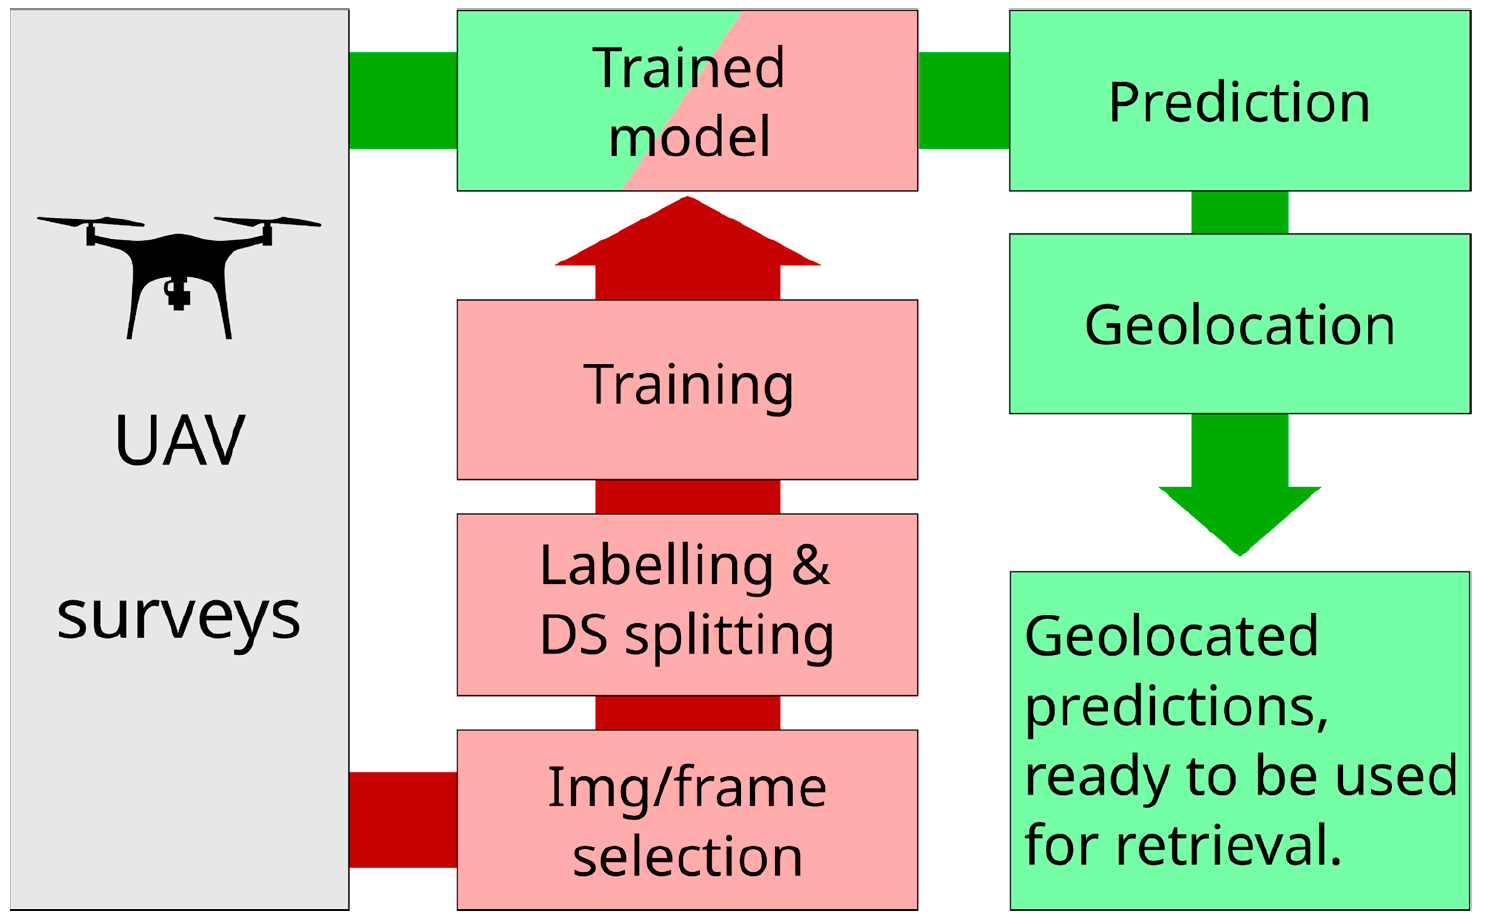
\includegraphics[width=0.7\linewidth]{beachlitter1.png}
    \caption{The system architecture of the real-time \gls{uav} beach litter monitoring and geolocation system, highlighting the two main pipelines: training (in red) and prediction (in green). (Source: \cite{beach_litter})}
    \label{fig:beachlitter1}
\end{figure}

% The authors also developed a geolocation algorithm to enhance the utility of the detected litter by integrating it with a robot for debris retrieval. For the algorithm to communicate the detection coordinates to the robot, the predictions made by the \gls{yolo}v5 model needed to be geolocated. This required that the original footage include \gls{gps} coordinates of the drone. The geolocation process involved several key steps: calculating the pixel size of the footage, determining the distance between meridians and parallels at the latitude of recording, measuring the horizontal and vertical distance from the prediction box's centre to the image centre, and transforming these distances into real-world coordinates. Figure \ref{fig:beachlitter2} shows the schematic for calculating litter geolocations, highlighting the parameters used to map the detected litter to real-world coordinates. To improve accuracy, the authors also calculated the distance between each litter object and the camera’s field of view, factoring in variables such as the \gls{uav}’s height and the angle of the camera’s lens. This enabled precise localisation of litter in both the image and the real-world environment, essential for guiding the robot to specific debris \cite{beach_litter}.

% \begin{figure}[!htbp]
%     \centering
%     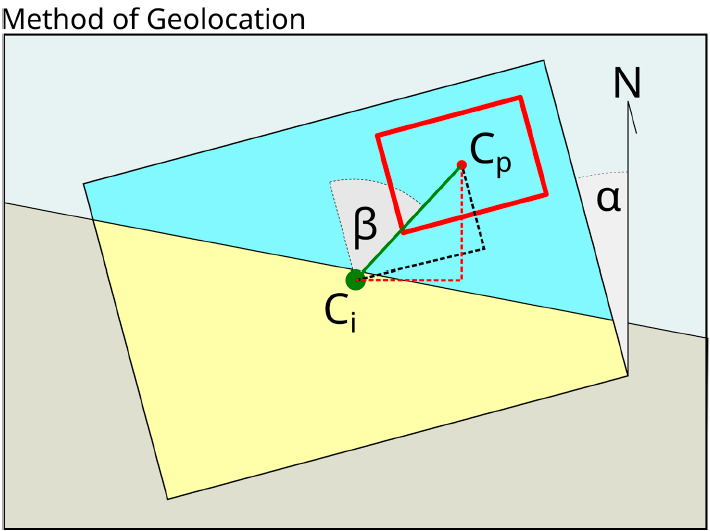
\includegraphics[width=0.7\linewidth]{beachlitter2.png}
%     \caption{Schematic representation of the calculation of litter geolocations, illustrating the parameters used to map the detected litter to real-world coordinates. (Source: \cite{beach_litter})}
%     \label{fig:beachlitter2}
% \end{figure}
The authors also created a geolocation algorithm to link detected litter with a debris-retrieving robot, requiring that detection coordinates be translated into real-world positions. This process used \gls{gps}-tagged footage and involved calculating pixel dimensions, spatial distances, and converting image offsets into geographic coordinates. Accuracy was further refined by incorporating \gls{uav} height and camera angle, ensuring reliable localisation for robotic retrieval \cite{beach_litter}.
The results of their experiments using the \gls{yolo}v5 model on the labelled dataset were as follows: precision of 0.695, recall of 0.288, \gls{map}@50 of 0.314, and \gls{map}@50-95 of 0.2. The model performed most reliably on the following ten classes: \textit{plastic bottle}, \textit{metal can}, \textit{plastic bottle} \textit{cap}, \textit{plastic container}, \textit{shoe}, \textit{cardboard}, \textit{pop tab}, \textit{rope \& string}, \textit{wood}, and \textit{glass bottle} \cite{beach_litter}.

\subsection{TrashNet: Real-Time Object Detection for Trash Classification}
\label{subsec:3_trashnet}

In 2024, Veeravadivel Santhanalakshmi, and Nguyen introduced TrashNet, an object detection model designed to classify images of waste in real time. The dataset employed to train the TrashNet network comprises six primary categories of litter: \textit{cardboard}, \textit{glass}, \textit{metal}, \textit{paper}, \textit{plastic}, and \textit{general waste}. This dataset, derived from an image classification dataset on Kaggle, does not utilise \gls{uav}-based data. The TrashNet dataset comprises 2,524 annotated images, each featuring a single object instance. In addition, the authors explain that the dataset was divided into three subsets for model development: 70\% for training, 20\% for testing, and 10\% for validation.
In this study, the \gls{yolo}v5 object detection model was used, and its performance was evaluated using using metrics such as mean \gls{map}, precision, recall, and F1 score. 
The authors highlight that the primary aim of this study was to develop a real-time system to assist individuals in identifying the correct bin for various types of waste near rubbish disposal areas, as seen in Figure \ref{fig:trashnet}. Notably, the model successfully fulfilled this objective, achieving an accuracy of 90\% on both the validation and testing sets \cite{trashnet}.

\begin{figure}[!htbp]
    \centering
    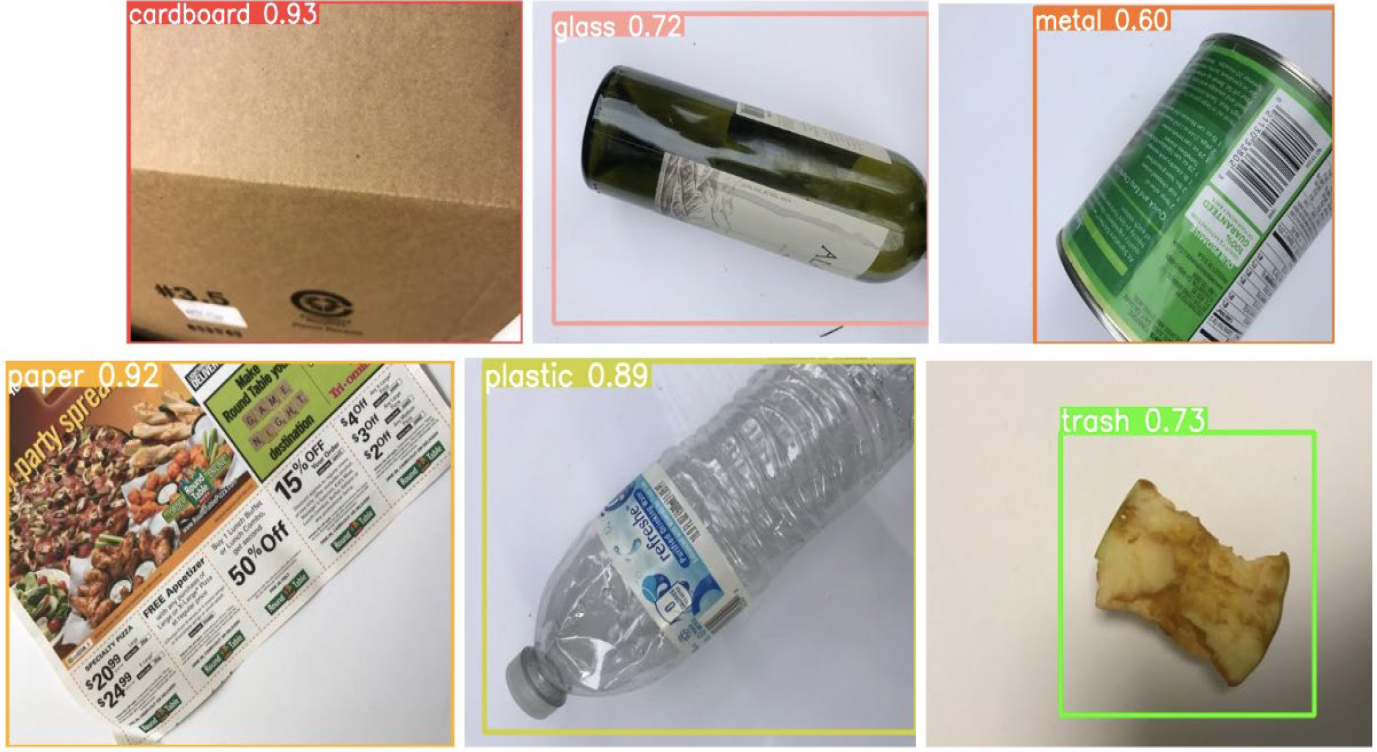
\includegraphics[width=0.7\linewidth]{trashnet.png}
    \caption{Litter detection results generated by the TrashNet detection model. (Source: \cite{trashnet})}
    \label{fig:trashnet}
\end{figure}

\subsection{SODA: Small Objects at Different Altitudes}
\label{subsec:3_sodadataset}

Modern \gls{uav}s are equipped with high-resolution cameras capable of capturing detailed pictures and videos of their surroundings. However, when the \gls{uav} is flying at higher altitudes, objects in the images may look very tiny, occupying only a few pixels. This poses substantial hurdles for spotting such objects. To tackle this issue, Pisani et al. (2024) introduced the \gls{soda} dataset, designed to aid research focused on small object detection in aerial imagery \cite{soda_dataset}. The dataset features six primary types of litter, derived from the \gls{taco} dataset: \textit{clear plastic bottles}, \textit{other plastic bottles}, \textit{glass bottles}, \textit{glass jars}, \textit{drinking cans}, and \textit{drinking cartons}. Figure \ref{fig:soda1} illustrates examples of litter categories used in the \gls{soda} dataset. Furthermore, the images were collected using a combination of DJI Mini 2 and DJI Air 2S UAVs at various altitudes, including 1m, 5m, 10m, 15m, 20m, 25m, and 30m \cite{soda_dataset, detect_litter}.

\begin{figure}[!htbp]
    \centering
    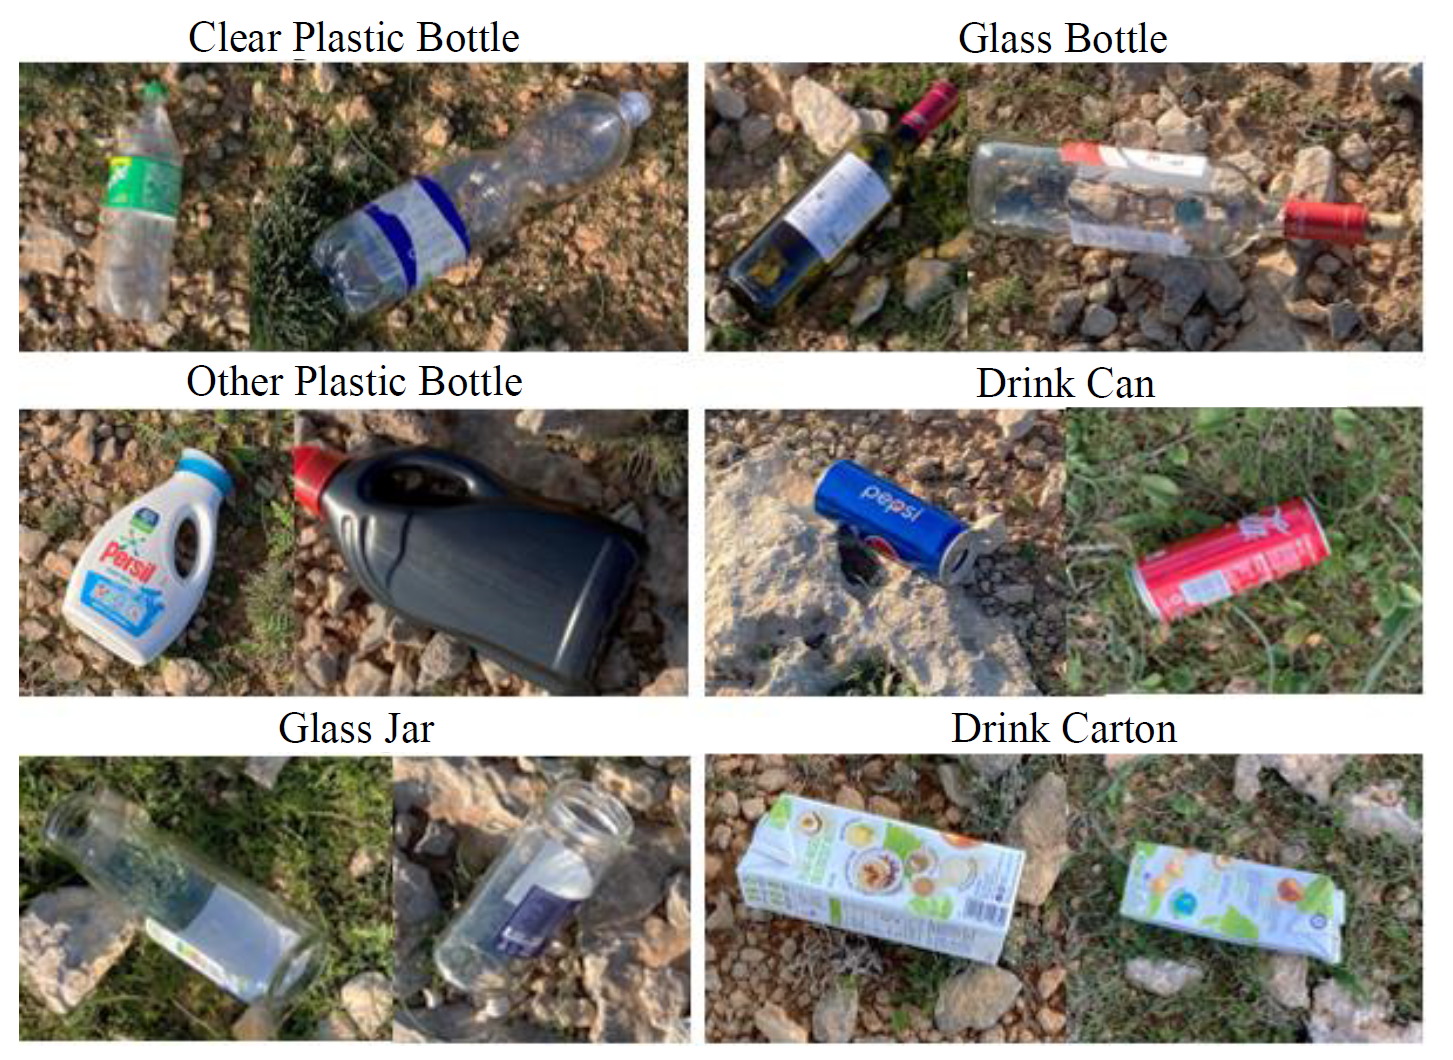
\includegraphics[width=0.8\columnwidth]{soda_images.png}
    \caption{The six object categories featured in the SODA dataset. (Source: \cite{soda_dataset})}
    \label{fig:soda1}
\end{figure}

The \gls{soda} dataset consists of 829 annotated images, with 452 (54.52\%) taken at 1 metre and 377 (45.48\%) captured from altitudes of 5 metres or more. 
The \gls{soda} dataset supports multi-class classification, with each object annotated with a distinct label using polygons rather than bounding boxes. The authors explain that polygons offer a more accurate fit around the object, whereas bounding boxes often capture additional background. Additionally, they clarify that polygons provide precise alignment during augmentations, such as rotation. Techniques for annotating with polygons and applying these augmentations are outlined in \cite{mask_to_annotation}. However, although the \gls{soda} dataset is annotated using polygons, the authors focus on the challenge of object detection rather than instance segmentation.
To address the challenge of detecting small objects across multiple categories of litter, the authors employed three different training strategies. The first approach involved segregating the training dataset according to altitude. In the second approach, the dataset was merged while maintaining multi-class labels. The third approach also merged the dataset but consolidated all categories into a single \textit{litter} class. 
Notably, a key feature of this study was the application of a \textit{tiling methodology} to improve the detection of small objects. This technique divides an image into a grid and splits it into smaller, equally sized sections, which were used in both the training and inference stages. The authors note that the grid size can significantly influence detection performance, with smaller grids, such as $2 \times 2$ (refer to Figure \ref{fig:soda2}), used at lower altitudes and larger grids, like $5 \times 5$, applied at higher altitudes. For the \gls{soda} dataset, a $5 \times 5$ grid was used across all altitudes and images \cite{detect_litter, soda_dataset, daniel_thesis}.

\begin{figure}[!htbp]
    \centering
    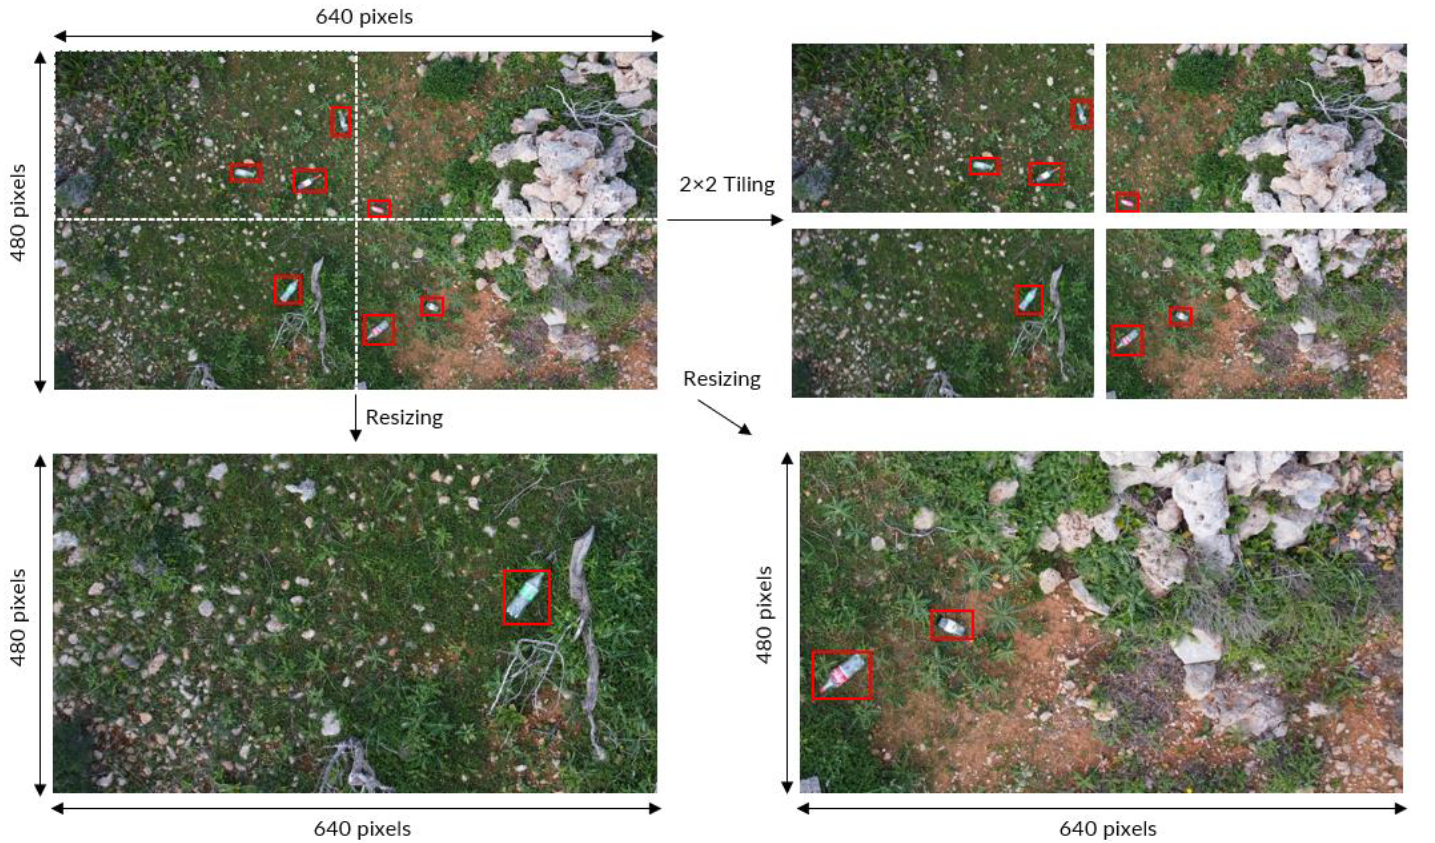
\includegraphics[width=0.9\columnwidth]{soda2.png}
    \caption{Application of a $2 \times 2$ tiling grid to aerial imagery captured at an altitude of 5 metres. (Source: \cite{detect_litter})}
    \label{fig:soda2}
\end{figure}

Three object detection models were trained for this study: \gls{yolo}v5 and \gls{yolo}v8 (both one-stage detectors) and Faster \gls{rcnn} (a two-stage detector). Models trained using the second and third approaches were evaluated on the \gls{bdw} dataset. The results indicated that the third approach, which merged all classes into a single litter category, outperformed the second approach. Additionally, the evaluation revealed that the \gls{soda} dataset was lacking a sufficient number of images of clear plastic bottles. 
In terms of \gls{map}, the results for the different models were as follows: Faster \gls{rcnn} achieved a \gls{map} of 0.921, \gls{yolo}v5 had a \gls{map} of 0.854, and \gls{yolo}v8 performed with a \gls{map} of 0.728 \cite{soda_dataset, detect_litter}. 
Finally, this study contributes to the use of \gls{uav}s for capturing aerial imagery and applying computer vision techniques to detect and classify objects within these images. The authors emphasise its significance as a crucial phase and a stepping stone towards the automation of litter collection for cleanup efforts \cite{detect_litter, soda_dataset, daniel_thesis}.

\subsection{Discussion}
\label{subsec:3_discussion}

The reviewed datasets and approaches highlight the growing potential, and popularity of \gls{uav}-based \gls{ai} systems for litter detection and management. While certain datasets were originally developed for recycling classification in indoor or controlled settings, others target outdoor environments, which present significantly greater challenges. Datasets that rely on \gls{uav}s are particularly affected by the difficulty of identifying small objects from aerial perspectives.
The variation across datasets reveals a wide range of technical and contextual difficulties associated with litter detection, as shown in Table \ref{tab:lit_review}. For example, datasets such as TrashNet \cite{trashnet}, MJU-Waste \cite{mju_waste}, and ZeroWaste \cite{zerowaste} were created under artificial conditions. In contrast, datasets like PlastoPol \cite{plastopol}, TACO \cite{taco2020}, and several \gls{uav}-oriented collections \cite{haida,soda_dataset,uavvaste,bdwdataset,beach_litter,superdock,umgeosurvey} contain real-world data collected in natural and urban environments.

Honing in on \gls{uav}-based litter deteciton, a recurring limitation evident in \gls{uav} datasets is the restricted number of annotated categories. In many cases, only one category is included. To this end, when multiple categories are included in a dataset, a common practice observed was to conduct an experiment by merging all classes into a single general litter category. Another challenge lies in the height at which data are collected. Most \gls{uav}-based datasets capture images at around 10 metres \gls{agl} or less. Exceptions such as \gls{bdw} \cite{bdwdataset} and \gls{soda} \cite{soda_dataset} extend this altitude to 30 metres, while the Beach Litter Dataset \cite{beach_litter} reaches up to 60 metres. Notwithstanding this, from among the \gls{uav} litter datasets only the \gls{soda} dataset \cite{soda_dataset} provides altitude-specific subsets of data.
Notably, the diversity of litter datasets and public accessibility is a key factor in supporting further development of \gls{ai}-based litter detection systems. Although several of the reviewed datasets have been featured in international peer-reviewed conferences and journals, only a limited number are available to the public. As illustrated in Table \ref{tab:lit_review}, the publicly accessible datasets include \gls{bdw} \cite{bdwdataset}, \gls{taco} \cite{taco2020}, MJU-Waste \cite{mju_waste}, UAVVaste \cite{uavvaste}, ZeroWaste \cite{zerowaste}, PlastoPol \cite{plastopol}, HAIDA \cite{haida}, TrashNet \cite{trashnet}, and \gls{soda} \cite{soda_dataset}, with just four of these specifically developed for \gls{uav} applications.

In terms of detection methods, \textit{data augmentation} is frequently employed to improve model performance. This is a common practice across both \gls{uav} and ground-based approaches. Techniques such as image \textit{tiling} or \textit{slicing} are especially important to facilititate \gls{uav}-based litter detection. High-resolution drone footage, often recorded in 4K, provides greater visual detail, which helps in identifying smaller objects. However, standard object detection models typically require downscaled inputs, ranging between $640$ and $1280$ pixels. This reduction can enable small litter objects even harder to detect. Splitting the original image into smaller tiles helps to preserve object size and minimise the loss of pixel detail. Nevertheless, proper experimentation of this method must be ensured, as adopting this process increases the computational load.

% Table \ref{tab:lit_review} presents a systematically organised comparison of the datasets and approaches, highlighting that the three primary challenges addressed were object detection, instance segmentation, and object geolocation, spanning both \gls{uav}-based and non-\gls{uav} datasets. It is also evident that for \gls{uav}-based approaches, altitudes ranging from 10 metres to 30 metres were the most commonly used. Additionally, in terms of the number of categories or litter types represented across datasets, both \gls{uav} and non-\gls{uav} approaches predominantly focus on creating single-class labelled datasets, with a few exceptions, such as recent approaches employing 6 to 10 classes, excluding the Beach Litter \cite{beach_litter} and \gls{taco} \cite{taco2020} datasets. Additionally, despite non-UAV datasets often containing a relatively large number of images, most \gls{uav}-based datasets consist of a smaller number of images, with notable exceptions being the \gls{bdw} \cite{bdwdataset} and Beach Litter \cite{beach_litter} datasets.

\begin{table*}[htbp]
\centering
\scriptsize
\begin{adjustbox}{max width=\textwidth, center}
\renewcommand{\arraystretch}{2.0}%1.5
\begin{tabular}{|l|c|c|c|c|c|c|c|}%|l|l|
\hline
\textbf{Name} & \textbf{Year} & \textbf{No of. Images} & \textbf{UAV}& \textbf{AGL Altitudes} & \textbf{Dataset Details}& \textbf{No of. Categories}  & \textbf{Available}\\ 
\hline \hline
BDW Dataset \cite{bdwdataset} & 2018 & 25,407 & Yes & 10m--30m & Detection & 1 (Litter)  &Yes\\ \hline
UM Geo. Survey \cite{umgeosurvey} & 2018 & 472 & Yes & 30m & Data Collection & 5 (Litter)  &No\\\hline
SuperDock \cite{superdock} & 2019 & 100 & Yes & 5m--10m & Detection & 1 (Litter)  &No\\\hline
Styrofoam Monitoring \cite{styrofoam} & 2019 & N/S\footnotemark[1] & Yes & 15m & Detection, Segmentation & 1 (Litter)  &No\\\hline
Small Litter Detection \cite{small_litter_detection} & 2019 & 744 & Yes & 5m--10m & Detection & 1 (Litter)  &No\\\hline
TACO Dataset \cite{taco2020} & 2020 & 1,500 & No & N/A\footnotemark[2] & Detection, Segmentation & 60 (Litter) [28 Super]  &Yes\\\hline
MJU-Waste Dataset \cite{mju_waste} & 2020 & 2,475 & No & N/A\footnotemark[2] & Segmentation & 1 (Litter)  &Yes\\\hline
UAVVaste Dataset \cite{uavvaste} & 2021 & 772 & Yes & low-altitude & Detection, Geolocation & 1 (Litter)  &Yes\\\hline
ZeroWaste Dataset \cite{zerowaste} & 2022 & 10,715 & No & N/A\footnotemark[2] & Detection, Segmentation & 4 (Litter)  &Yes\\\hline
PlasOPol Dataset \cite{plastopol} & 2022 & 2,418 & No & N/A\footnotemark[2] & Detection & 1 (Litter)  &Yes\\\hline
HAIDA Dataset \cite{haida} & 2022 & 1,319 & Yes & 1m--10m & Detection, Geolocation & 2 (Litter)  &Yes\\\hline
Bangladeshi Dataset \cite{bangladeshi} & 2023 & 4,418 & No & N/A\footnotemark[2] & Detection & 10 (Litter)  &No\\\hline
Beach Litter Dataset \cite{beach_litter} & 2023 & 4,126 & Yes & 10m--60m & Detection, Geolocation & 67 (Litter) [7 Super]  &No\\\hline
TrashNet \cite{trashnet} & 2024 & 2,524 & No & N/A\footnotemark[2] & Detection & 6 (Litter)  &Yes\\\hline
SODA Dataset \cite{soda_dataset} & 2024 & 829 & Yes & 1m, 5m--30m & Detection, Segmentation & 6 (Litter) [4 Super]  &Yes\\\hline
\end{tabular}
\renewcommand{\arraystretch}{1}
\end{adjustbox}
\caption{Comparison of datasets and approaches, systematically organised, with litter-related images captured from both \gls{uav} and non-\gls{uav} data.}
\label{tab:lit_review}
\end{table*}

\footnotetext[1]{N/S: The amount of images was not specified.}
\footnotetext[2]{N/A: Not applicable for non-\gls{uav}-based litter detection datasets.}

In addressing the problem of litter detection, most studies rely on deep learning models. The most commonly used architectures include variants of \gls{yolo} \cite{yolo, yolov5, yolov8}, along with Faster \gls{rcnn} \cite{fasterrcnn}, RetinaNet \cite{retinanet}, \gls{ssd} \cite{ssd}, and EfficientDet \cite{efficientdet}. A typical approach involves using these general object detection models as out-of-the-box solutions for the task \cite{soda_dataset, detect_litter, plastopol, beach_litter}. Other studies, such as those by \cite{small_litter_detection, styrofoam}, have explored modifications to the architecture and incorporated techniques such as background removal and \gls{cam} to improve results.
Additionally, some methods \cite{taco2020, mju_waste, zerowaste} approach the problem not just as an object detection problem but also as one of litter instance segmentation. In this regard, models like DeepLabv3 \cite{deeplabv3} and Mask \gls{rcnn} \cite{maskrcnn} have gained prominence. Interestingly, other \gls{uav}-based approaches \cite{beach_litter,haida,uavvaste} aim to address litter geolocation or georeferencing. These methods develop algorithms based on drone properties and mathematical formulas, allowing integration with the detection outputs to determine the precise locations of the detected litter.


\section{Review of Learning Using Privileged Information in Computer Vision}
\label{subsec:2_lupi}
% Glorja lil Missier u lil-iben u lil-Ispirtu Santu, Kif kien mill-bidu issa ghal dejjem ta' dejjem. Amen. Salve Regina
At the time of writing this dissertation, no prior research has applied the \gls{lupi} paradigm within the problem of object detection. The most closely related work lies within the broader field of computer vision, where the application of \gls{lupi} remains relatively sparse. In this domain, many tasks exhibit an asymmetry in the availability of information between the training and testing phases \cite{learning2rank}, rendering \gls{lupi} particularly relevant.

Sharmanska et al. \cite{learning2rank, learning2rank2} explore four distinct forms of privileged information for image classification: semantic attributes, bounding boxes, textual descriptions, and annotator rationale. Their experiments apply these types of privileged information within a rank transfer framework compatible with SVM solvers, focusing on the SVM+ algorithm. Their findings indicate a measurable improvement in classification performance when \gls{lupi} is integrated into the learning process \cite{learning2rank, learning2rank2}.
In a related contribution, Wang et al. \cite{lupi_classification} also address multi-label image classification by incorporating privileged information during training. Their approach employs similarity constraints derived from privileged inputs, along with ranking constraints informed by multiple labels, to develop a more effective classifier. High-resolution images and associated image tags serve as the privileged data, available solely during training. The method is evaluated across several benchmark datasets, and the results suggest that the inclusion of privileged information, alongside an awareness of label dependencies, contributes meaningfully to improved model performance \cite{lupi_classification}.

Although not directly related to \gls{lupi}, a substantial body of work aligns conceptually through the use of knowledge distillation techniques within computer vision \cite{distillation1, distillation2}. Knowledge distillation is a prominent method in machine learning, facilitating the transfer of information from a high-capacity model to a smaller, more efficient counterpart \cite{hinton_distillation}. This process enables the distilled model to retain essential predictive capabilities while reducing computational overhead.

In the context of vision-based tasks, various distillation methods have been explored, including those based on output responses, internal feature representations, and inter-feature relationships \cite{distillation1}. These techniques are applicable across a range of visual domains, including image classification, object detection, and multimodal frameworks. Specific to object detection, two widely adopted strategies are feature imitation and logit matching, which aim to replicate intermediate activations and output distributions respectively \cite{distillation2}.
A particularly noteworthy development is the concept of localisation distillation, as proposed in \cite{distillation2}, which refines the transfer process by concentrating on spatial regions deemed informative for both classification and localisation. This targeted distillation allows the student model to better capture salient visual patterns by selectively attending to regions that contribute meaningfully to detection accuracy.

\section{Conclusion}
\label{sec:2_conclusion}
% Sliema ghalik Marija, bil Grazzja Mimlija, Imbierek il frott tal guf tieghek Gesu', Qaddisa Marija Omm Alla, itlob ghalina il midinbin, issa u fis siegha tal mewt taghna. Amen.

This chapter has provided a structured foundation for understanding the task of object detection, describing its core challenges and progressing through the evolution of methodologies, from traditional techniques to contemporary deep learning models. It has also outlined the conceptual basis and definition of the learning using privileged information framework, highlighting its potential to address information asymmetries during training by incorporating privileged data and distilling knowledge effectively. The discussion then turned to existing approaches in litter detection, considering both aerial and ground-based methods, as well as the broader application of \gls{lupi} within computer vision. Collectively, these sections provide the necessary foundation for a focused examination of how models trained using the \gls{lupi} framework may improve both the performance and robustness of litter detection systems.

% Grazzi Sinjur Alla, Ahfirli Sinjur Alla, u Ismaghni Sinjur Alla. Grazzi Hafna. Amen
%--

%-- Formatting Rules (Don't delete):

% \clearpage

% Figure~\ref{fig:sample} shows a sample figure and how to cross-reference
% figures.
% %
% \begin{figure}[htbp]
%     \centering
%     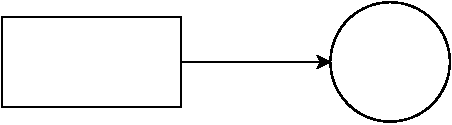
\includegraphics[width=\textwidth,keepaspectratio]{sample}
%     \caption[Short sample caption.]{Longer caption that  and shows below the figure.\label{fig:sample}}
% \end{figure}
% %
% Lorem ipsum dolor sit amet, consectetur adipiscing elit.
% Mauris sed ipsum risus.
% Nulla aliquet quis quam sed eleifend.
% Donec rutrum, dolor id vulputate pharetra, nulla tortor laoreet nisl,
% pellentesque dapibus velit dolor suscipit purus.
% Phasellus vitae eleifend sem.
% Integer ultricies ex in neque pellentesque, vitae facilisis orci aliquam.
% In pellentesque mollis turpis, eu tristique lacus eleifend nec.
% Vestibulum orci neque, rhoncus vitae convallis eu, suscipit quis dui.
% Nulla libero elit, porta sit amet sagittis vel, placerat sit amet tortor.
% Aliquam hendrerit dolor sit amet sollicitudin ornare.
% Aliquam placerat sodales est, in vestibulum nisl efficitur in.
% Nulla venenatis aliquam sem, at volutpat nisl pellentesque eleifend.
% Praesent vitae euismod nulla, eget vehicula turpis.
% Duis quis tellus vitae nisi tempus tincidunt.

% \section{Literature Review}%
% \label{sec:literature_review}

% Vivamus sit amet orci erat.
% Morbi eleifend velit purus, sed gravida metus ullamcorper sed.
% Aliquam sit amet interdum nulla, in aliquam diam.
% Aliquam non libero tortor.
% Nulla imperdiet dolor vel justo semper, ut efficitur enim varius.
% Donec ultrices odio id orci fringilla tristique.
% Ut fringilla nec felis a finibus.
% Sed a felis sed odio elementum porta a ac nisl.
% Curabitur suscipit, sem et facilisis tempus, nisl elit vestibulum eros, in
% varius dolor enim vitae ante.
% Vestibulum ante ipsum primis in faucibus orci luctus et ultrices posuere cubilia
% curae; Nullam condimentum tempor consectetur.
% Aliquam non porta nisi.
% Proin molestie tincidunt tellus, id varius nibh finibus eget.

% Vestibulum et neque erat.
% Curabitur metus velit, dictum non vehicula vitae, sodales sed purus.
% In mattis a mauris nec imperdiet.
% Duis volutpat mi eget egestas placerat.
% Vivamus non purus erat.
% Cras quis egestas libero.
% Sed id diam at enim vehicula porttitor.

% Mauris tincidunt elementum porttitor.
% Curabitur eu elit et metus luctus ultrices.
% Aenean varius orci in turpis consectetur efficitur.
% Quisque lacinia sagittis pharetra.
% Aliquam efficitur aliquam arcu, vel ullamcorper tortor volutpat nec.
% Curabitur sit amet semper tortor.
% Vestibulum ante ipsum primis in faucibus orci luctus et ultrices posuere cubilia
% curae; Cras at leo aliquet, porta mauris nec, pharetra augue.
% Nam volutpat eu urna in ullamcorper.
% Aliquam ultrices condimentum odio id eleifend.
% Mauris tellus felis, mattis et pellentesque ac, laoreet vitae eros.
% Aliquam at nisl lorem.
% Quisque consequat ligula nec tellus ornare eleifend.

% \section{Instructions}%
% \label{sec:instructions}

% This sentence refers to Section~\ref{sec:literature_review}, as an example of
% how to do cross-referencing.
% Equation~\eqref{eq:emc} shows one of the most famous equations.
% %
% \begin{equation}
%     \label{eq:emc}
%     e = mc^2
% \end{equation}
% %
% An example of how to create multiple equations, where they all align is given
% below.
% %
% \begin{align}
%     e & = mc^2          \\
%     m & = \frac{e}{c^2}
% \end{align}

% \section{Inserting references}%
% \label{sec:inserting_references}

% To insert a reference, the entry must be inserted in the \texttt{references.bib}
% file.
% The key or unique ID of the entry is then used to refer to it.
% \LaTeX{} will automatically number the entry and generate the list of
% references.
% The paper in~\cite{sample_key} is used as a referencing example.

% \section{Inserting acronyms}%
% \label{sec:inserting_acronyms_and_glossary_entries}

% The \gls{tcp} and \gls{udp} protocols are two layer 4 protocols, used for
% demonstrating how to use acronyms.
% On the second use of an acronym, only its initials are shown as demonstrated in
% the following sentence.
% The \gls{tcp} and \gls{udp} protocols are two layer 4 protocols, used for
% demonstrating how to use acronyms.

% \section{Using glossary terms}%
% \label{sec:using_glossary_terms}

% Let \gls{G} represent a loop-free directed graph, where \gls{V} and \gls{E}
% represent the set of nodes and edges, respectively.

% \section{Inserting a table}%
% \label{sec:inserting_a_table}

% A simple table is shown in Table~\ref{tab:simple}, with a more complex example
% given in Table~\ref{tab:complex}.

% \begin{table}
%     \caption{Simple table example.\label{tab:simple}}
%     \centering
%     \begin{tblr}{|c|S[table-format=3.2]|c|}
%         \hline
%         \textbf{Header 1} & \textbf{Header 2} & \textbf{Header 3} \\
%         \hline
%         1                 & 2.3               & Orange            \\
%         2                 & 100.5             & Blue              \\
%         3                 & 35.0              & Black             \\
%         \hline
%     \end{tblr}
% \end{table}

% \begin{table}
%     \centering
%     \caption{Complex table example.\label{tab:complex}}
%     \begin{tblr}{|Q[m,0.2\textwidth]|Q[m,0.2\textwidth]|Q[m,0.2\textwidth]|Q[m,0.2\textwidth]|}
%         \hline
%         \SetCell[r=2]{c} Table Head & \SetCell[c=3]{c} Table Column Head & & \\
%         \hline
%         & Table column subhead 1 & Table column subhead 2 & Table column subhead 3 \\
%         \hline
%         Item 1 & 2 & 3 & 4 \\
%         \hline
%         Item 2 & 2 & 3 & 4 \\
%         \hline
%         Item 3 & 2 & 3 & 4 \\
%         \hline
%         Item 4 & 2 & 3 & 4 \\
%         \hline
%     \end{tblr}
% \end{table}

% \section{Inserting code snippet}%
% \label{sec:inserting_code_snippet}

% The code snippet in Listing~\ref{lst:python_example} demonstrates a very simple
% python program.

% \begin{lstlisting}[language=Python,caption=Python example,label={lst:python_example}]
% def main() -> None:
%     print("Hello World")

% if __name__ == "__main__":
%     main()

% # Comment
% \end{lstlisting}

% \section{Inserting theorems, corollaries and lemmas}%
% \label{sec:inserting_theorems,_corollaries_and_lemmas}

% \begin{theorem}
%     Let \(f\) be a function whose derivative exists in every point, then \(f\) is
%     a continuous function.
% \end{theorem}

% \begin{theorem}[Pythagorean theorem]
%     \label{pythagorean}
%     This is a theorem about right triangles and can be summarised in the next
%     equation
%     \[ x^2 + y^2 = z^2 \]
% \end{theorem}

% And a consequence of theorem \ref{pythagorean} is the statement in the next
% corollary.

% \begin{corollary}
%     There's no right rectangle whose sides measure 3cm, 4cm, and 6cm.
% \end{corollary}

% You can reference theorems such as \ref{pythagorean} when a label is assigned.

% \begin{lemma}
%     Given two line segments whose lengths are \(a\) and \(b\) respectively there is a
%     real number \(r\) such that \(b=ra\).
% \end{lemma}

% \section{Inserting an algorithm}%
% \label{sec:inserting_an_algorithm}

% The pseudocode for a basic \gls{ea} using NSGA-II is given in
% Algorithm~\ref{alg:evolutionaryAlgorithm}.

% \begin{algorithm}
%     \caption{Pseudocode for an Evolutionary Algorithm}%
%     \label{alg:evolutionaryAlgorithm}
%     \begin{algorithmic}
%         \State \( \mathcal{P} \) = Population Size
%         \State \( \chi \) = Number of Generations
%         \State \( \omega \) = Crossover Probability
%         \State \( \psi \) = Mutation Probability
%         \State
%         \State population = GenerateInitialPopulation(\( \mathcal{P} \))
%         \For{\( 1, 2, \ldots, \chi \)}
%         \State offspring = TournamentSelection(population, \( \mathcal{P} \))
%         % Crossover
%         \For{\(c_i \in \) offspring, \( i = 1, 3, 5, \ldots, \mathcal{P}\)}
%         \State \(z\) = random(0, 1)
%         \If{\( z < \omega \)}
%         \State Crossover(\( c_i, c_{i+1} \))
%         \EndIf
%         \EndFor
%         % Mutation
%         \For{\(c_i \in \) offspring}
%         \State \(z\) = random(0, 1)
%         \If{\( z < \psi \)}
%         \State Mutate(\( c_i \))
%         \EndIf
%         \EndFor
%         % Calculate fitness
%         \State CalculatePopulationFitness(offspring)
%         % Update population size
%         \State population = NSGA-II([population + offspring], \(\mathcal{P}\))
%         \EndFor
%     \end{algorithmic}
% \end{algorithm}
